\chapter{Anden Iteration}
I dette afsnit beskrives 2. iteration af design- og implementeringsfasen. Den indebærer design og vikling af transformator samt valg af resterende komponenter i kredsløbet. Yderligere realiseres og testes hele kredsløbet for første gang i 2. iteration.

\section{Transformator}
Transformeren fungerer anderledes ved en flyback end ved de fleste andre SMPS, hvor der løber en strøm i de primære og sekundære viklinger på samme tid. Det er ikke tilfældet ved en flyback konstruktion. Her løber strømmen kun i en vikling af gangen. Når MOSFET’en er on, vil strømmen igennem den primære vikling rampe op i forhold til indgangsspændingen og induktansen i viklingen. Pga. dioden og polariteten af den sekundære vikling, vil der på dette tidspunkt, ikke løbe en strøm i den vikling. Når transistoren går off falder strømmen i den primære vikling til 0, som får spændingerne over viklingerne til at skifte polaritet. Med en modsat polaritet på sekundærsiden, kan der nu løbe en strøm gennem dioden. 


\noindent Normalt kan energien fra den primære vikling transformeres direkte over i den sekundære vikling, da der løber en strøm på samme tid. Da det ikke er tilfældet ved flyback, kræver konstruktionen, at transformeren kan opbevare energien fra den primære vikling, indtil det kan transformeres over i den sekundære vikling. Det gør at der i transformeren er behov for et air gap, for at transformeren ikke skal gå i mætning. 


\noindent Det er fluxændringen i kernen, der sørger for, at der induceres spænding over i den sekundære vikling. Det vil sige, at der er behov for at fluxen i kernen ændrer sig forholdsvis lineært, hvilket sker når der ligger en konstant spænding over viklingen. Kernen siges at have nået mætning, når en ændring i H-feltet ikke længere ændrer lineært på fluxen. 


\noindent For at sikre ens transformatoren ikke går i mætning bruges hysteresekurven (ses på figur~\ref{fig: Hysteresekurve}) som plotter H-feltet på x aksen og B-feltet op ad y aksen. Her skal det undgås at transformatoren kommer til at blive vandret i top eller bund, da det er her, at transformatoren går i mætning. Yderligere fås et overblik over selve transformatortabet ud fra samme kurve. Det areal, som kurven indeholder, er nemlig tabet i transformatoren per switchperiode. Det betyder ligeledes, at kernetabet bliver større jo højere switch frekvens der benyttes. 

\begin{figure}[H]
	\center
	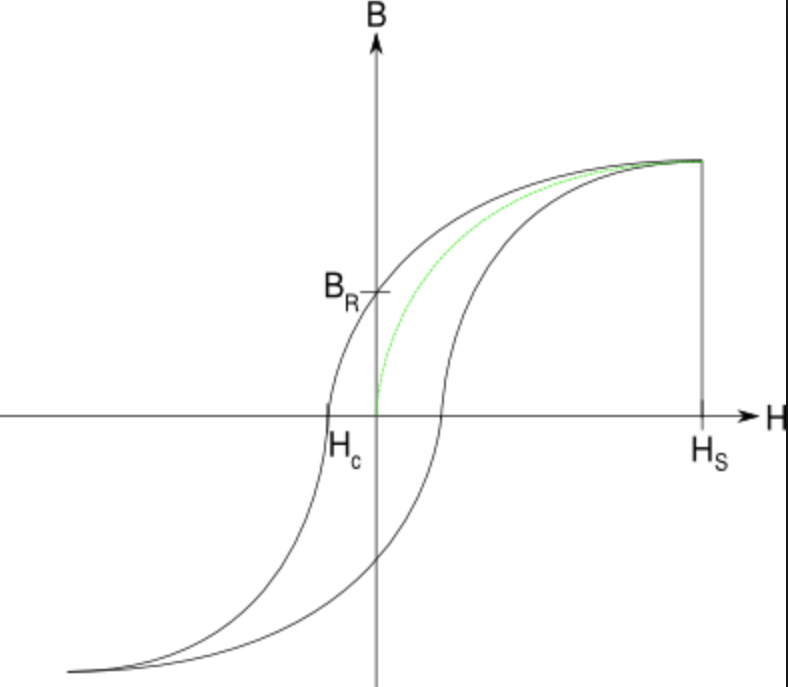
\includegraphics[max width=0.7\linewidth]{/tex/2iteration/billeder/Hysteresekurve.png}
	\caption{Hysteresekurve}
	\label{fig: Hysteresekurve}
\end{figure}
\textbf{Tænker teorien her er lidt tynd, eller er det nok??}

\subsection{Design}
Først og fremmest findes ripplestrømmen, som skal løbe i transformatoren. Her er der taget udgangspunkt i, at designe den efter $60\percent$ af udgangsstrømmen. Dette er et tradeoff mellem størrelsen på ripplen og hvor høj en induktans vi får i viklingerne. Større induktans kræver flere vindinger og giver dermed mere tab.
\begin{equation} \label{I_ripple_CCM}
I_{ripple} = 0.6 \cdot \frac{V_{out} \cdot I_{out}}{V_{inmaks} \cdot   D_{min}} = 2.13A
\end{equation}
Den nødvendige induktans det kræver for at transformatoren kan rampe op til den nødvendige strøm inden for dutycyclen, udregnes på følgende måde:
\begin{equation} \label{L_CCM}
L = \frac{V_{inmin} \cdot D_{min}}{I_{ripple} \cdot f_s} = 69.43\micro H
\end{equation}
Som beskrevet tidligere skal kernen kunne opbevare den energi som kommer fra primær viklingen, når transistoren er on, for at undgå mætning. Mængden af energi i primærviklingen udregnes ved:
\begin{equation} \label{Primary_energy}
w = \frac{1} {2} \cdot L \cdot {I_{pk}}^2 = 1.083\milli J
\end{equation}
For at beregne den tilladelige mængde energi i transformatoren, skal kernen og kernematerialet kendes. Valget er her faldet på en RM8 kerne og materialet 3f3. RM8 kernens mål gør, at den lige akkurat kan være på printet højdemæssigt. Derudover har Terma tidligere brugt RM8 kerner med 3f3 og har nogle mere præcise mål på AL og air gaps, end der er på datasheets’ne. (Kræver det flere argumenter?)


\noindent Den effektive volumen Ve aflæses for RM8. På databladet for 3f3 aflæses et maks peak af B-feltet til omkring $250\milli T$. Hvis der designes efter, at transformatoren vil operere med et højere B-felt, vil man altså risikere at kernen går i mætning. Yderligere findes permeabiliteten for 3f3 materialet uden luftgap. Med disse oplysninger vil transformatoren kunne opbevare følgende energi:
\begin{equation} \label{Energy_no_gap}
w_{kerne} = \frac{1} {2} \cdot \frac{1}{\micro_e} \cdot B^2 \cdot V_e = 53\pico J
\end{equation}
Det er tydeligt at den nødvendige energi på ingen måde kan opbevares i kernen. Da ferrit kan opbevare så lidt energi som det er tilfældet, kan det estimeres at al energien vil blive opbevaret i det luftgap, der designes. Derfor kan permeabiliteten ses som $\micro_0$ i den nye beregning. Den effektive volumen deles op i luftgap og $Al$, så luftgapet kan isoleres. Med dette kan luftgapet beregnes: 
\begin{equation} \label{Airgap}
l_g = \frac{L \cdot {I_{pk}}^2 \cdot \micro_0}{B^2 \cdot A_0} = 690.98\micro m
\end{equation}
Med den ripplestrøm der i første omgang er benyttet, skal der bruges et air gap på ca. $691\micro m$. Den nærmeste air gaps værdi for 3f3 ligger på $488\micro m$ hvilket giver en Al på $160\nano H$. (Dette er ikke databladets værdi, men en værdi der er blevet givet fra Terma, som har testet databladets værdier til ikke at være korrekte.) Det vil ikke fungere, derfor udregnes en induktans, der passer til det air gap i stedet: 
\begin{equation} \label{L1}
L_1 = \frac{l_g \cdot B^2 \cdot A_0}{{I_{pk}}^2 \cdot \micro_0} = 49.035\micro H
\end{equation}
Med kendt Al og induktans kan vindingstallet beregnes. Da der i 2. iteration bruges en 1:1 transformator er dette både for primær og sekundær vikling:
\begin{equation} \label{N}
N = \sqrt{\frac{L_1}{A_L}} = 17.5 \approx 18
\end{equation}
Det passer fint med 18 viklinger på hver side, hvor induktansen igen bliver lidt anderledes når vindingstallet rundes op. 
\begin{equation} \label{L1}
L_2 = N^2 \cdot A_L = 57.76 \micro H
\end{equation}
Med fastlagt induktans kan ny ripple- og peak strøm beregnes.
\begin{equation} \label{I_ripple_CCM}
I_{ripple} = \frac{V_{inmin} \cdot D_{max}}{L_2*f_s} = 2.24A
\end{equation}
\begin{equation} \label{I_pk_CCM}
I_{pk} = \frac{V_{out} \cdot I_{out}}{V_{inmin} \cdot D_{maks}} + \frac{I_{ripple}}{2} = 5.64A
\end{equation}

\subsection{Simulering}
I Pspice er kernen og materialet afprøvet, hvor resten af kredsløbet har været med ideele komponenter, for at kontrollere strømme og B-H kurve. Her ses den pspice-model af kernematerialet som bruges:
\begin{figure}[H]
	\center
	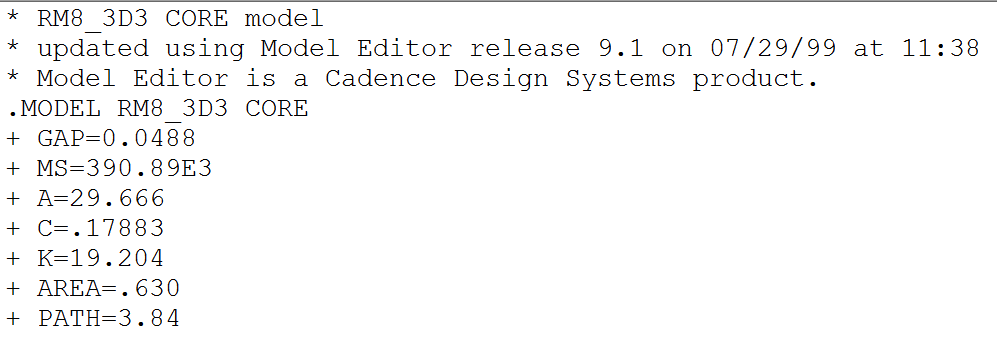
\includegraphics[max width=0.7\linewidth]{/tex/2iteration/billeder/Kernemodel.png}
	\caption{Kernemodel for RM8 3f3}
	\label{fig: Kernemodel}
\end{figure}
Kernemodellen for en 3f3 kerne er indsat, hvor det udregnede air gap også er indtastet. Derudover er der 19 vindinger på primær og sekundærspole. Ellers ingen ændringer i forhold til den rent ideele simulering. Først ses simuleringen af strømmene i transformatoren på primær og sekundær side.
\begin{figure}[H]
	\center
	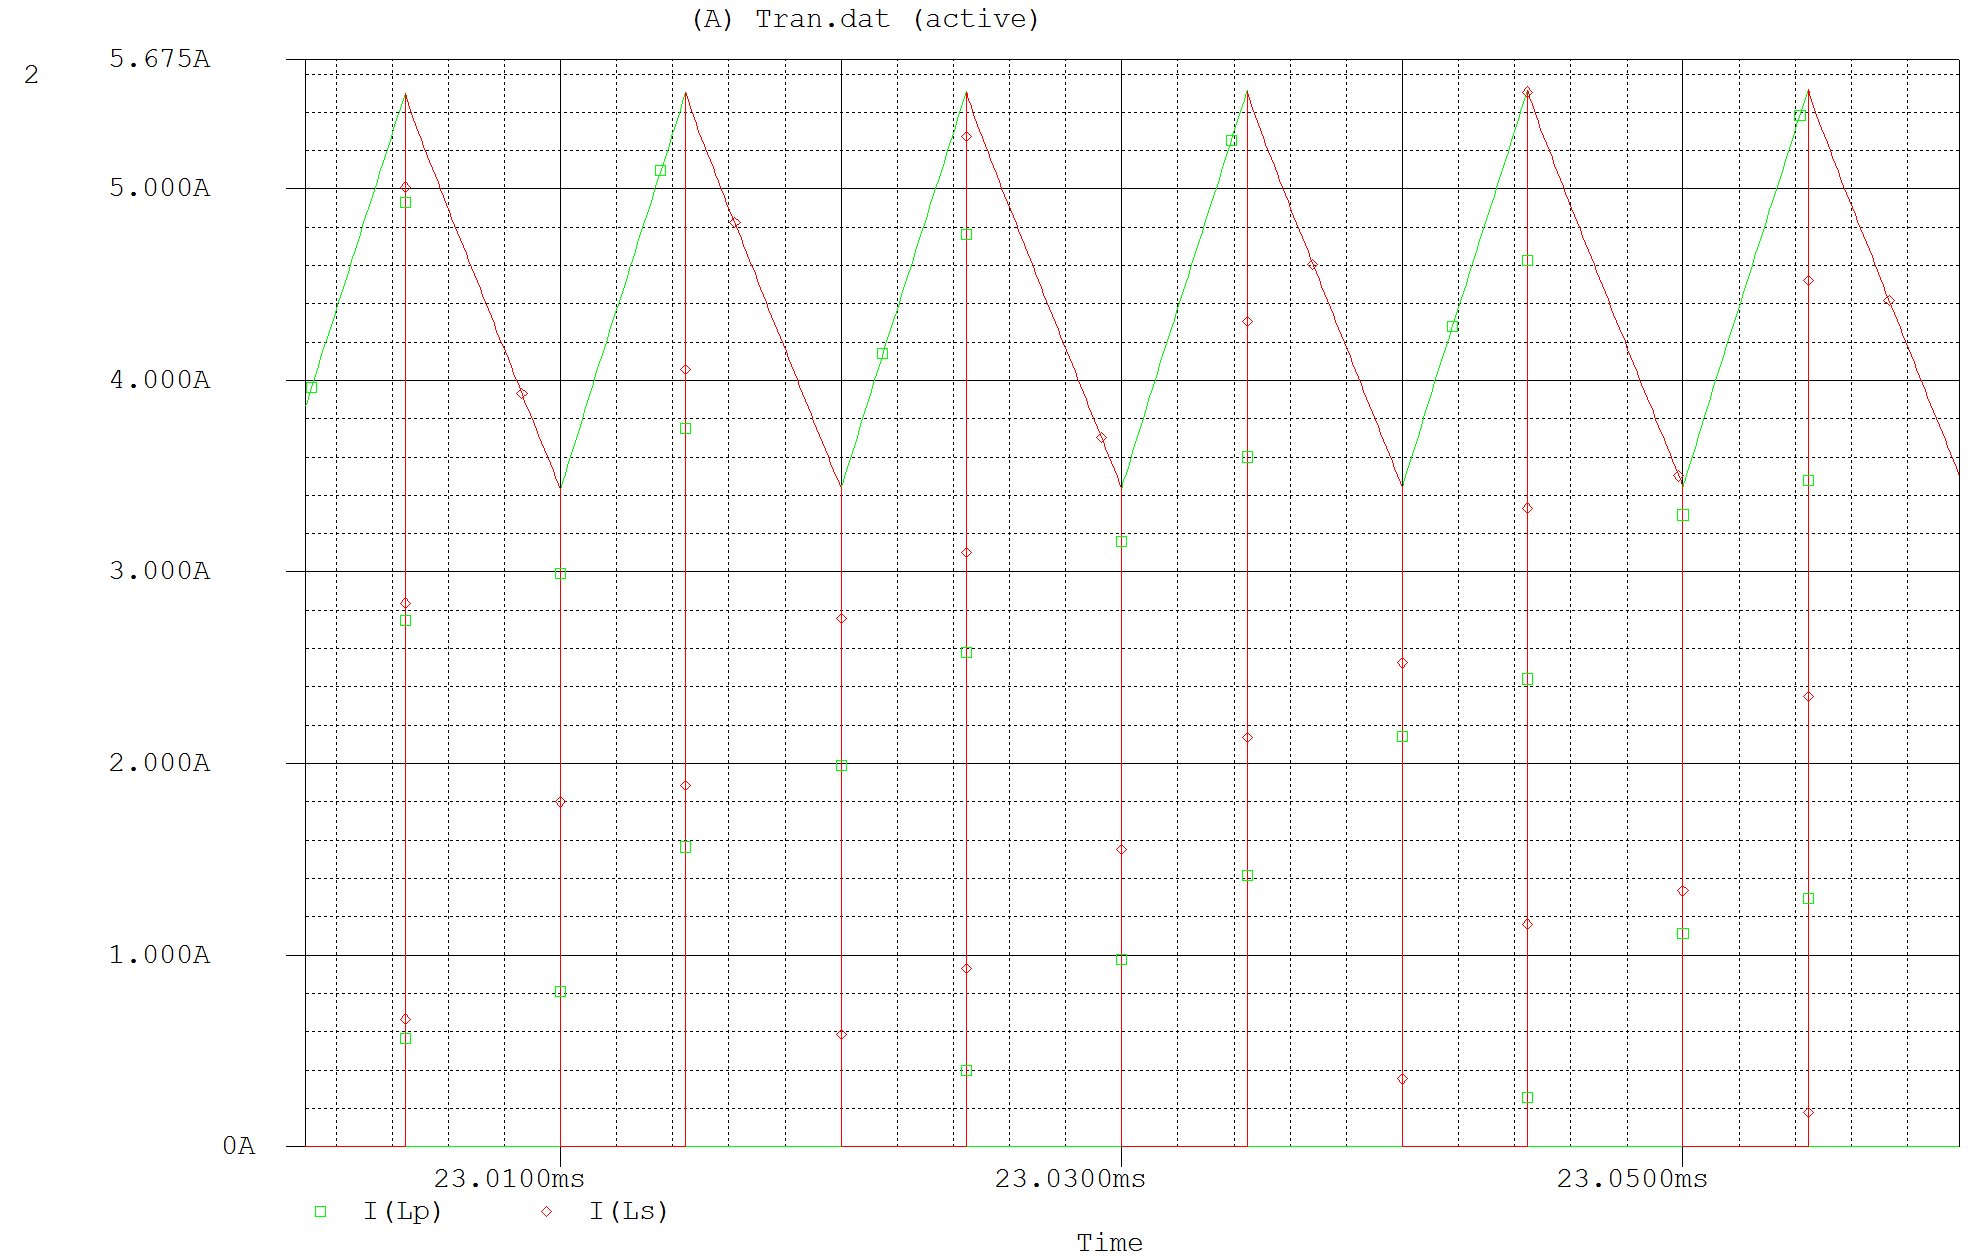
\includegraphics[max width=0.7\linewidth]{/tex/2iteration/billeder/Strom_pri_sek.png}
	\caption{Strøm i primær- og sekundærvikling}
	\label{fig: prisek_strom}
\end{figure}
Det ses tydeligt, at der som ventes køres i CCM, da ripplestrømmene ikke når ned til 0. Ripple- og peak strøm er, som det ses, ens for primær og sekundær, og aflæses til hhv. $2.27A$ og $5.69A$. Det passer fint med det udregnede på $2.24A$ og $5.64A$.
På figur~\ref{fig: RMS_trans} ses RMS strømmene:
\begin{figure}[H]
	\center
	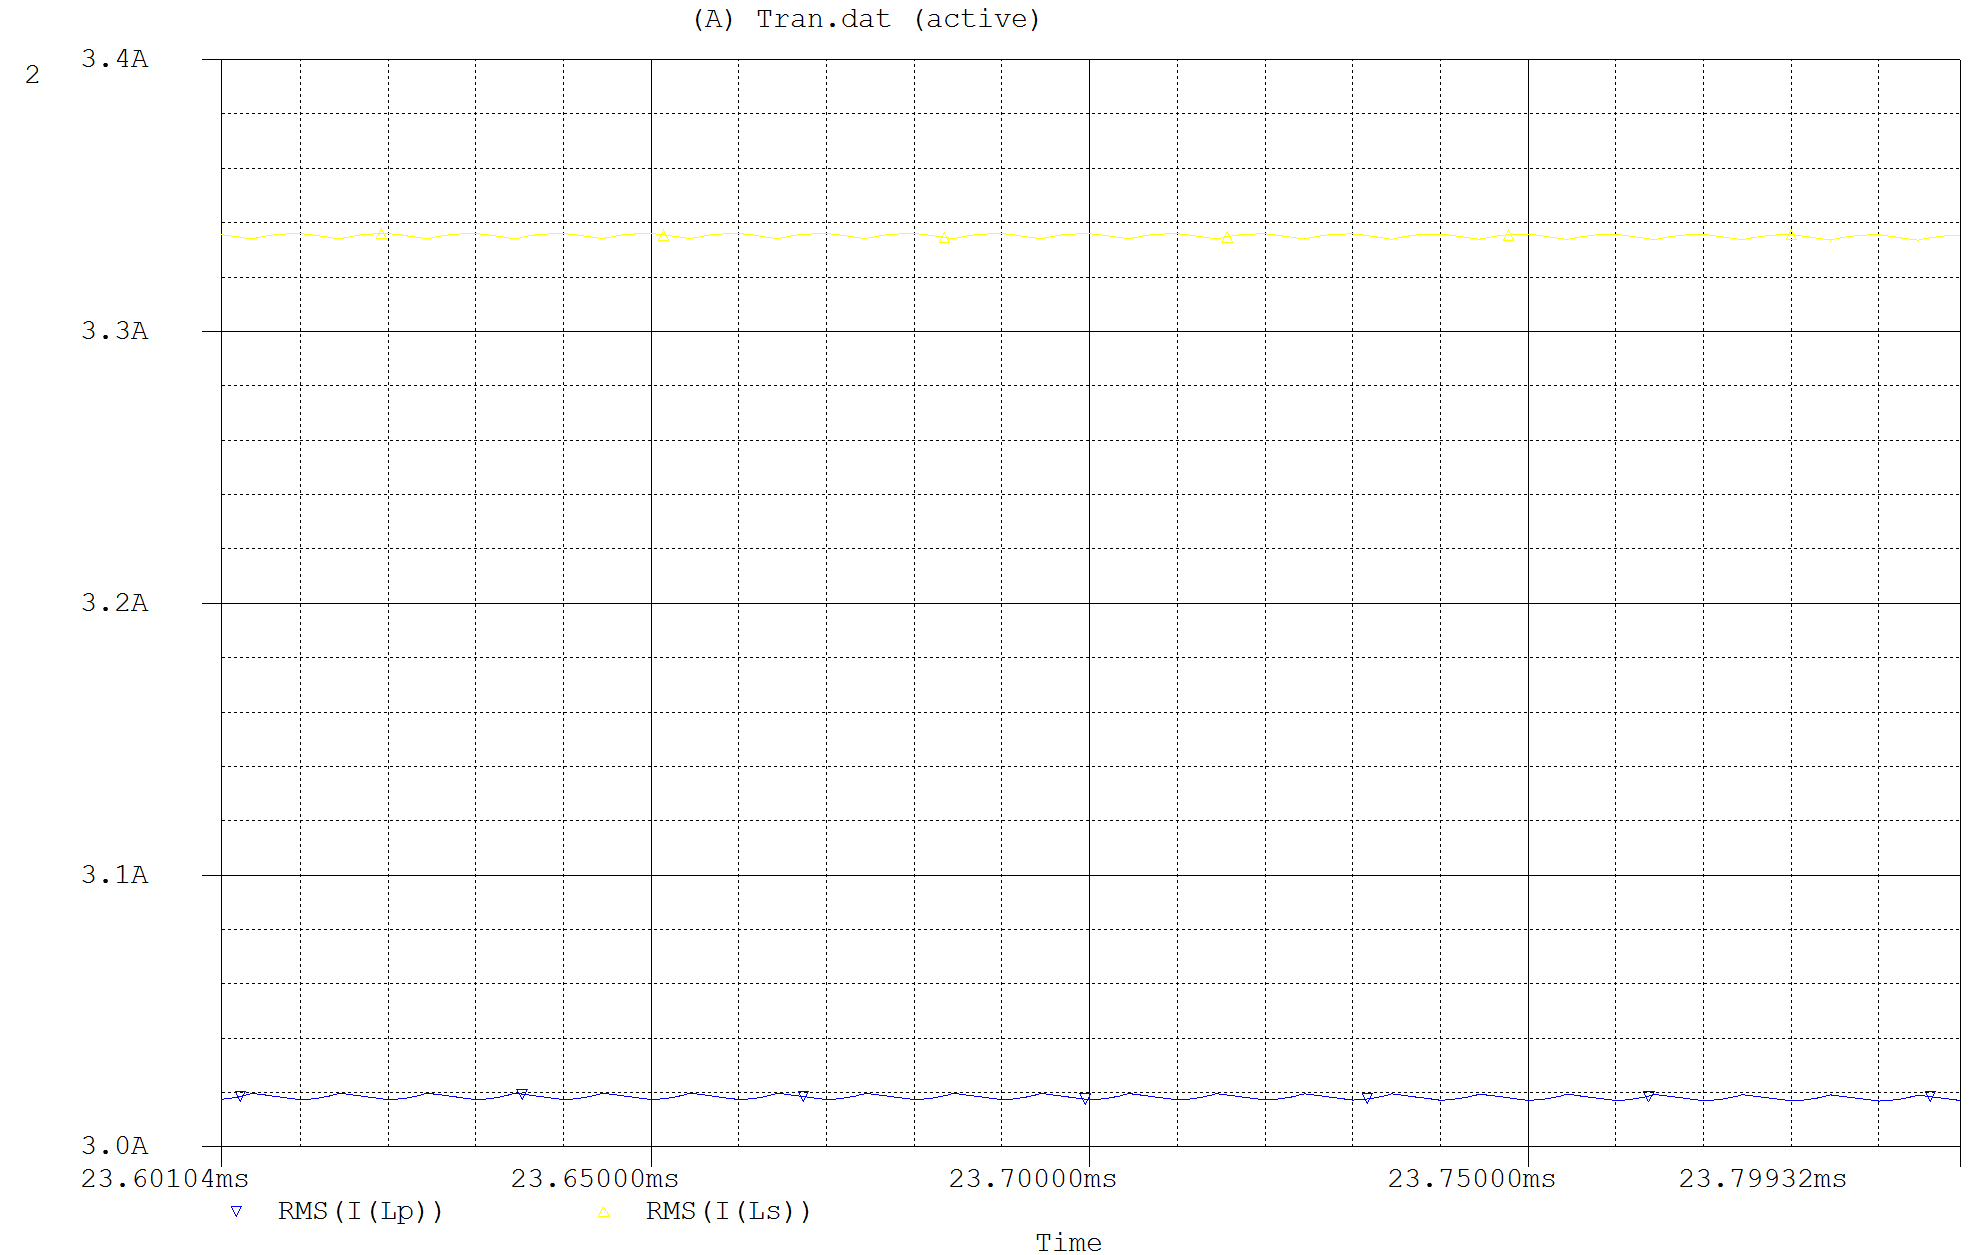
\includegraphics[max width=0.7\linewidth]{/tex/2iteration/billeder/RMS_transformator.png}
	\caption{RMS strømme i transformator (blå=primær og gul=sekundær)}
	\label{fig: RMS_trans}
\end{figure}
Her aflæses den primære til $3.01A$ og den sekundære til $3.33A$, hvilket igen stemmer godt overens med det beregnede på $3.02A$ og $3.36A$.


\noindent Herefter kigges på hysteresekurven, og sikres at den ikke kommer langt over de $250\milli T$, som der er designet efter:
\begin{figure}[H]
	\center
	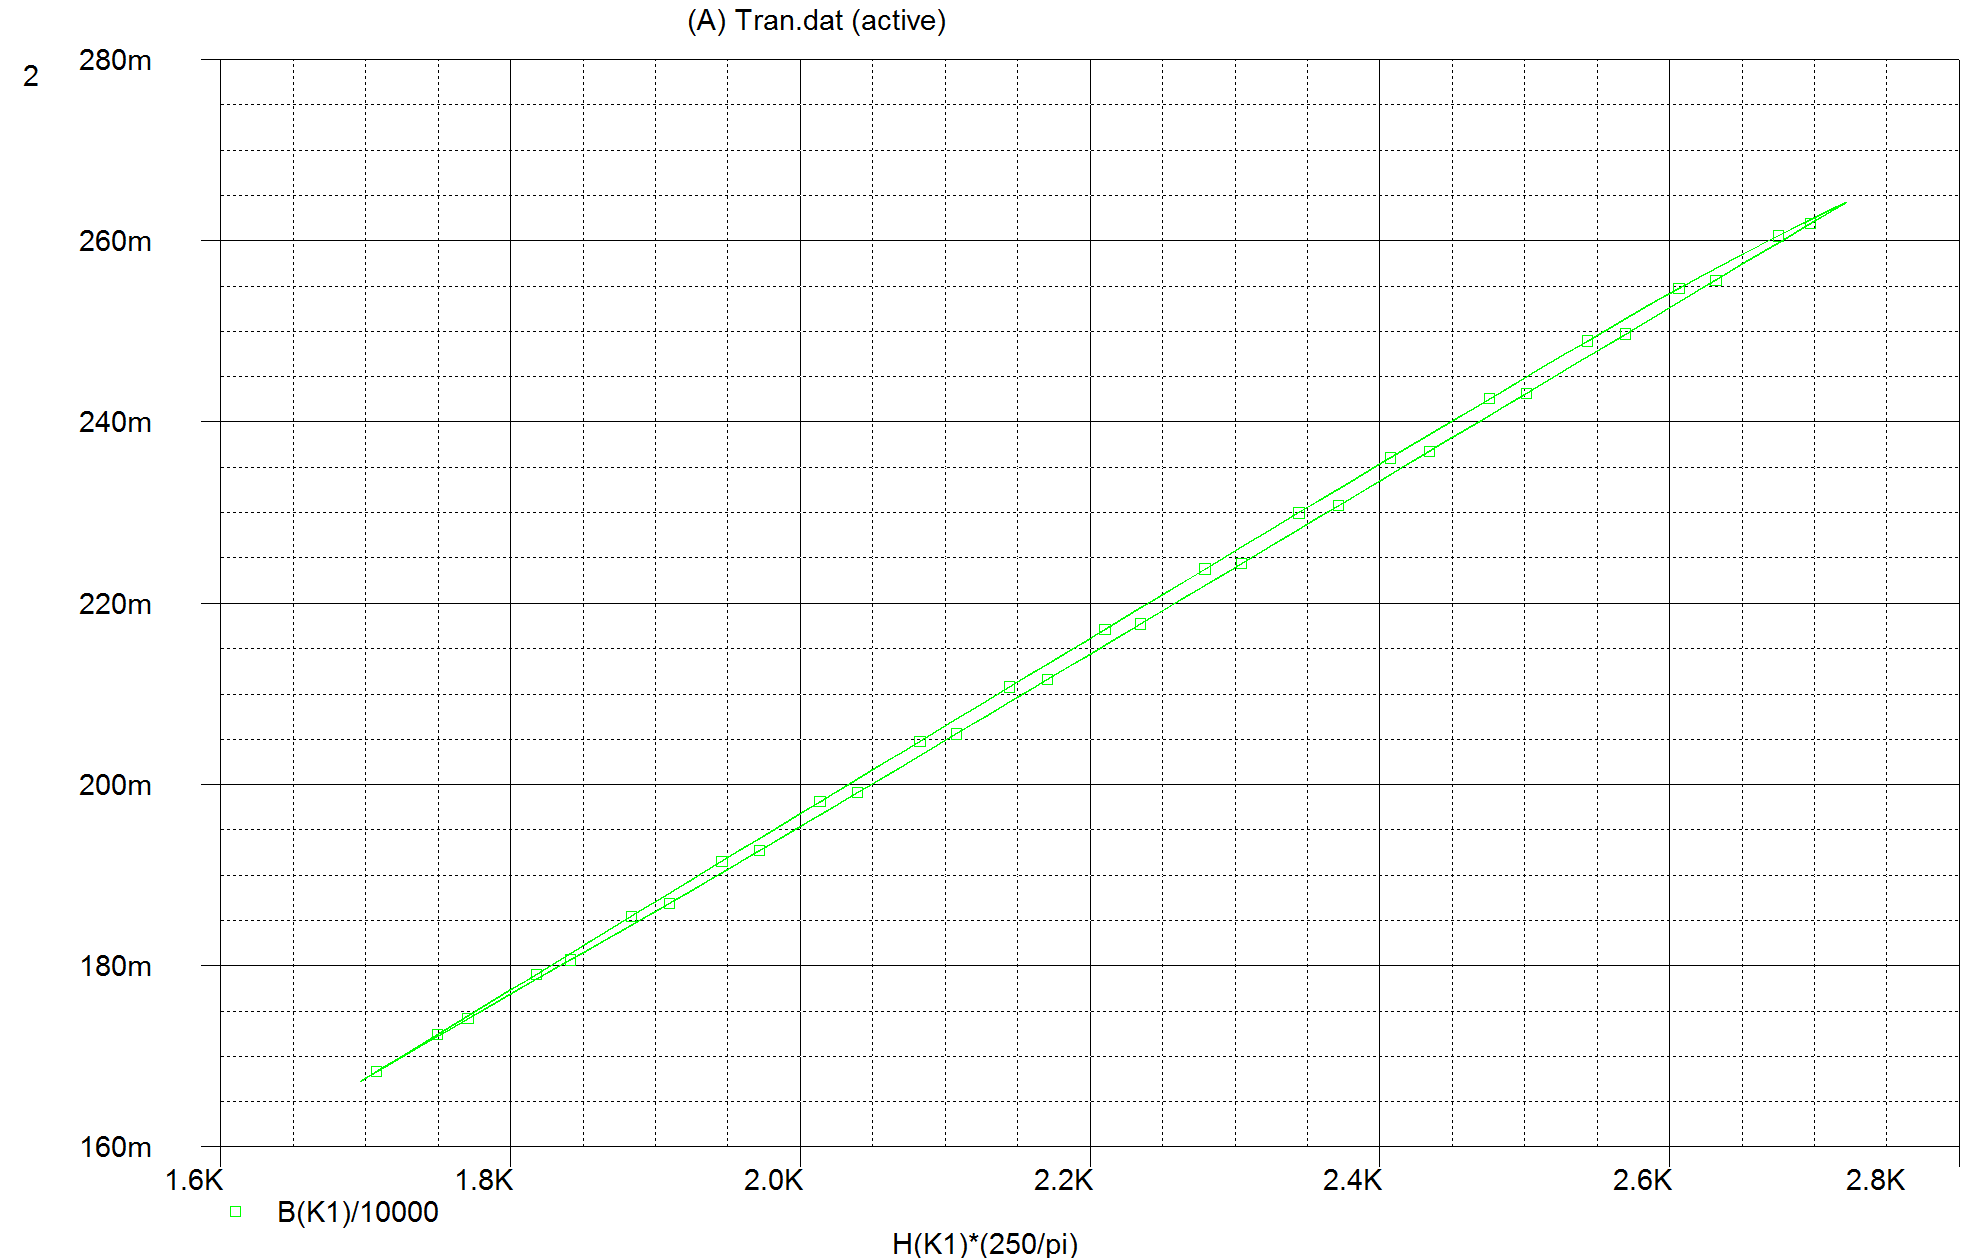
\includegraphics[max width=0.7\linewidth]{/tex/2iteration/billeder/Hysterese_trans.png}
	\caption{Hysteresekurve for transformatoren}
	\label{fig: Hysterese_trans}
\end{figure}
Peak fluxen ligger på ca. $265mT$ hvilket igen passer fint med det der er designet efter. Yderligere ville man kunne se i toppen og bunden af kurven, hvis den gik i mætning, hvilket den ikke gør her.
Tabet i selve kernen er simuleret ved at tage effekten ved den primære vikling i forhold til den sekundære vikling. Tages der i pspice en average af dette fås nedenstående kurve:
\begin{figure}[H]
	\center
	\includegraphics[max width=0.7\linewidth]{/tex/2iteration/billeder/tabkerne.png}
	\caption{Simuleret kernetab i transformator}
	\label{fig: Kernetab}
\end{figure}
Tabet er simuleret til at ligge ved ca. $310\milli W$

\subsection{Vikling af transformator}
Det er vigtigt at prøve at udnytte kernens mål fuldt ud når vindingerne vikles. Med RM8 kernen er der en bredde på $8.6\milli m$ og en højde på $3.475\milli m$. Ved 2. iteration forsøges de mål udnyttet bedst muligt.
Først udregnes den nødvendige diameter af tråden, når der skal ligge 18 vindinger per lag. 
\begin{equation} \label{d_trad}
d_{tråd} = \frac{8.6\milli m}{18} = 0.478\milli m
\end{equation}
Dette er dog den samlede diameter, altså inklusiv isolering. Der benyttes en isolering med grade 2, som giver en diameter på ledningen eksklusiv isolering på $0.425\milli m$.(HENVISNING) Transformeren er 1:1, så både primær og sekundær vikles med 18 vindinger per lag. Et lag af hver giver en højde på $0.956\milli m$. Altså ikke i nærheden af de $3.475\milli m$ i højden. Derfor vikles 2 ekstra viklinger i parallel for både primær- og sekundærsiden og får dermed den tredobbelte højde. Der indsættes tape mellem hver af de parallelle viklinger. Det giver samlet en højde på $2.867\milli m$ plus tape. Det giver i alt 6 lag, 3 for primær og 3 for sekundær. Overblikket over viklingen kan ses på nedenstående tegning:
\begin{figure}[H]
	\center
	\includegraphics[max width=0.7\linewidth]{/tex/2iteration/billeder/viklingsoverblik.png}
	\caption{Overblik over viklingsantal og tykkelse}
	\label{fig: viklingsoverblik}
\end{figure}
\noindent Tegnes bunden af transformatoren fås der et overblik over, hvordan viklingerne vikles. Det ses, at primær begynder og slutter i samme sidde af transformatoren, mens sekundær vikles fra den anden side.  
\begin{figure}[H]
	\center
	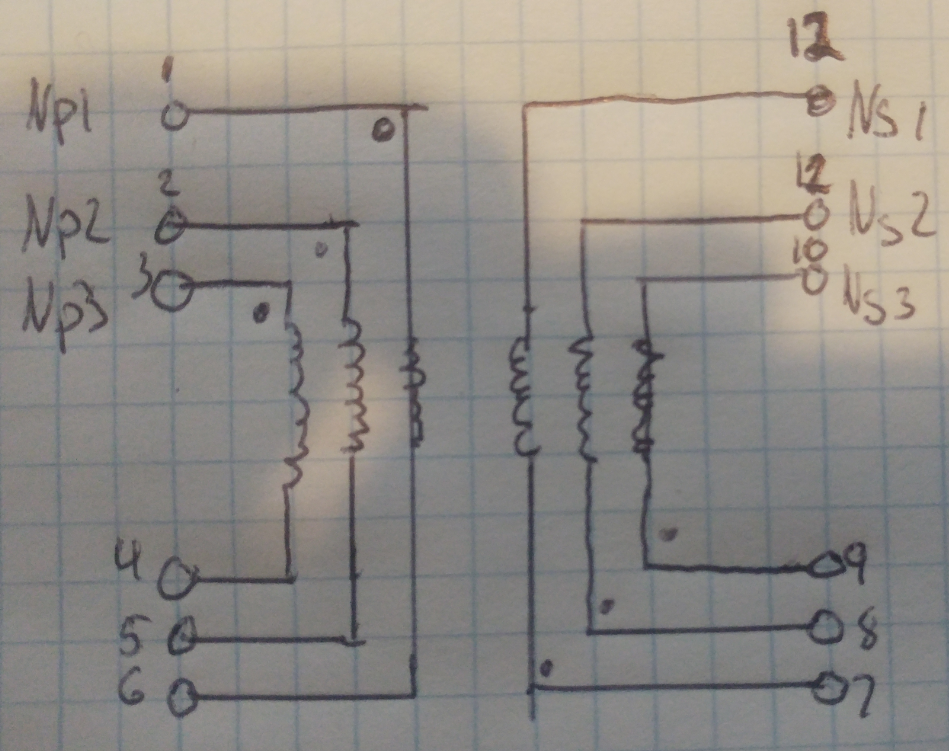
\includegraphics[max width=0.7\linewidth]{/tex/2iteration/billeder/Viklingsbegyndelse.png}
	\caption{Overblik over hvordan viklingerne vikles}
	\label{fig: viklingsbegyndelse}
\end{figure}
\noindent Sidste billede viser hvilken retning der vikles. Her vil primær og sekundær vikles modsatte vej af hinanden, for at få den modsatte polaritet som ønsket.
\begin{figure}[H]
	\center
	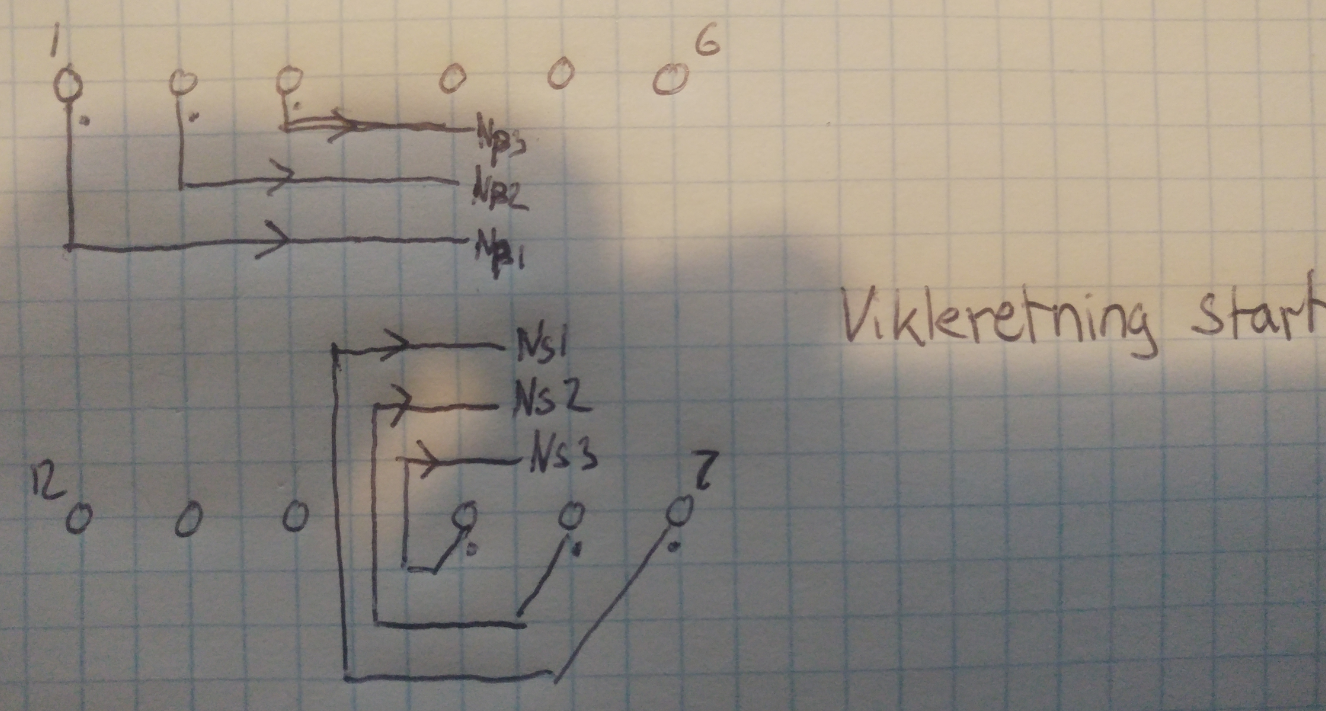
\includegraphics[max width=0.7\linewidth]{/tex/2iteration/billeder/Viklingsretning.png}
	\caption{Begyndelses retning for primær og sekundær}
	\label{fig: viklingsretning}
\end{figure}

\subsection{Realisering}
\begin{figure}[H]
	\center
	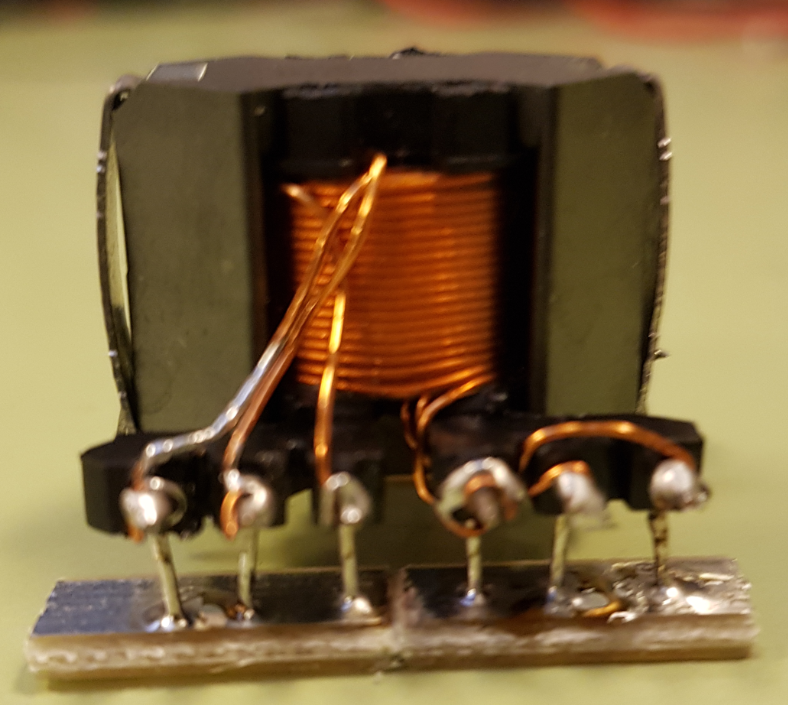
\includegraphics[max width=0.7\linewidth]{/tex/2iteration/billeder/Viklet_transformator.PNG}
	\caption{Viklet transformator}
	\label{fig: Viklettrans}
\end{figure}
På figur~\ref{fig: Viklettrans} ses den viklede transformator. Ved viklingen måtte det erkendes, at der ikke kunne presses 18 vindinger ind, med en ledningstykkelse på $0.450\milli m$, som ellers i forvejen var mindre end den udregnede tykkelse på $0.478\milli m$. I stedet benyttes en tykkelse på $0.425\milli m$ og der tilføjes en ekstra vikling, så det totale antal vindinger ender på 19 per vikling. (ER VI SIKRE PÅ DET IKKE NETOP ER DEN TRÅD VI HAR FÅET?? At trådtykkelsen der står er uden isolering?)

\noindent \textbf{Endelig induktans}


\noindent Da vindingstallet blev 19 i stedet for de 18, er induktansen lidt højere end beregnet i første omgang. Den endelige induktans den viklede transformator beregnes til:
\begin{equation} \label{L_2}
L_2 = N^2 \cdot A_L = 57.76\micro H
\end{equation}
Det ændrer igen en smule på ripple- og peak strømmen i transformatoren:
\begin{equation} \label{I_ripple_final}
I_{ripple} = \frac{V_{inmin} \cdot D_{max}}{L_2*f_s} = 2.01A
\end{equation}
\begin{equation} \label{I_pk_final}
I_{pk} = \frac{V_{out} \cdot I_{out}}{V_{inmin} \cdot D_{maks}} + \frac{I_{ripple}}{2} = 5.53A
\end{equation}

\subsection{Test af transformator}
Transformatoren er testet ved at måle både selvinduktionen i primær- og sekundærviklingerne samt spredningsselvinduktionen. Til dette blev en impedansmåler brugt. 


\noindent Til sådan en måling er det vigtigt, at gøre ledningerne så korte som muligt, da der vil skabes yderligere induktans i dem. Derfor ses ved opstillingen på figur~\ref{fig: Transopstilling} de meget korte ledninger samt at der bliver brugt en 4-wire teknik. Det vil sige to ledninger på hver side af det der måles på. Det gør at strømmen kan sendes igennem det ene sæt ledninger, mens der måles med det andet sæt. Da der ikke sendes en strøm igennem det sæt der måles på, undgås den induktive fejlmåling, der ellers vil komme fra ledningerne. 

\begin{figure}[H]
	\center
	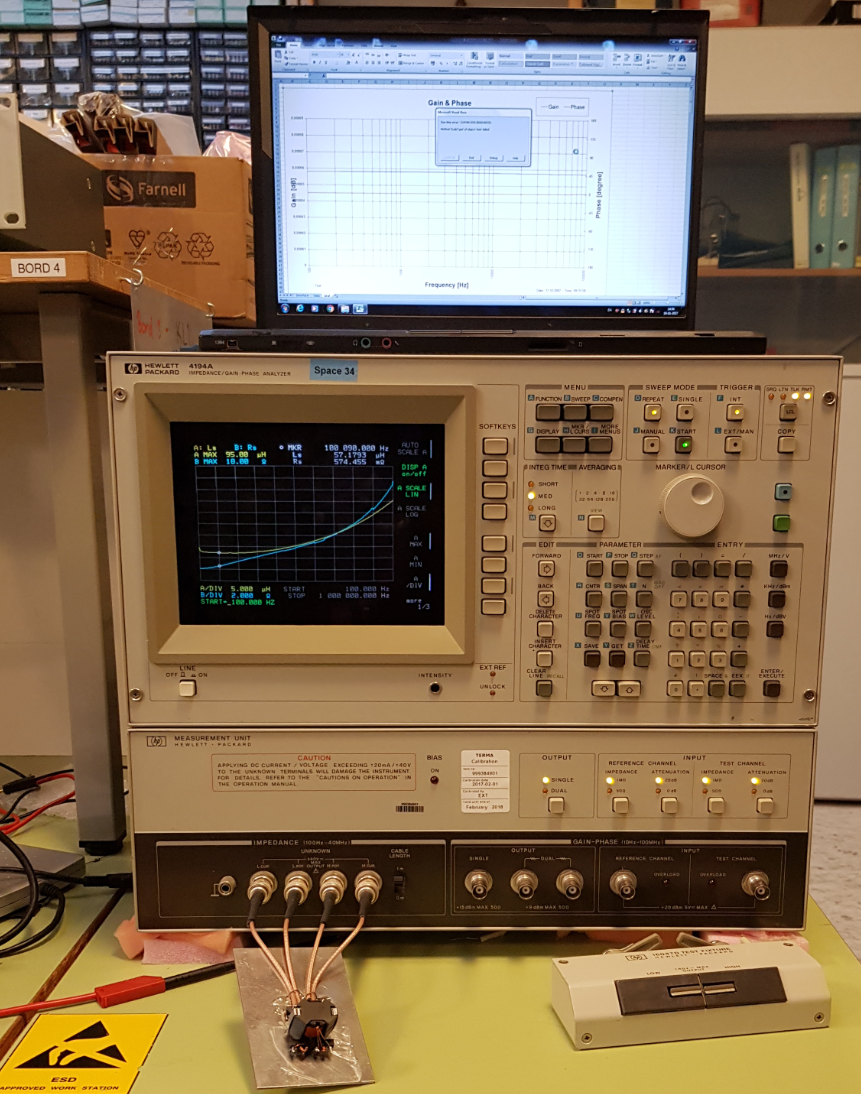
\includegraphics[max width=0.7\linewidth]{/tex/2iteration/billeder/Samlet_transformatortest_opstilling.PNG}
	\caption{Samlet transformatortest opstilling}
	\label{fig: Transopstilling}
\end{figure}

\noindent Måleresultaterne tages med USB ud af impedansmåleren og indsættes i et Excel ark.  

\noindent Selve impedansmåleren havde et lille offset på målingerne. Derfor blev der først lavet en kalibreringsmåling, hvor ledningerne alle målte samme sted. Offsettet herfra er i Excel trukket fra de efterfølgende målinger.    

\noindent Herefter måles der på de 2 sider af primærviklingen, mens sekundærsiden holdes åben. På denne måde fås induktansen i den primære vikling. Da transformatoren er 1:1, er det også induktansen i den sekundære vikling. 
\begin{figure}[H]
	\center
	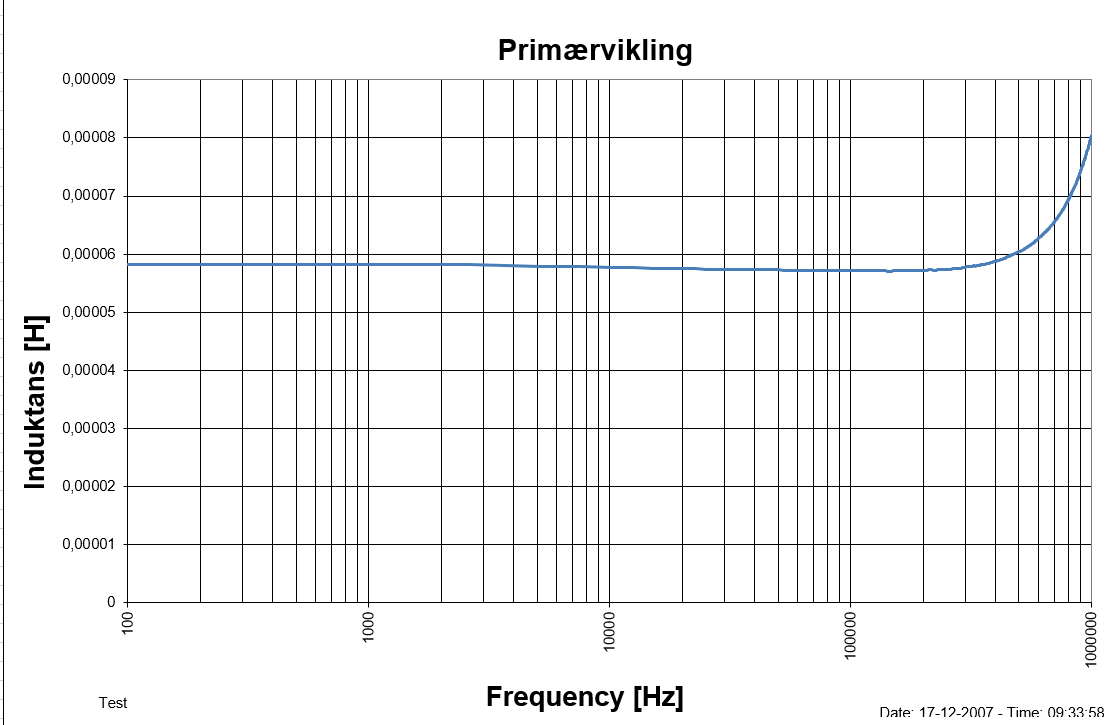
\includegraphics[max width=0.7\linewidth]{/tex/2iteration/billeder/Primarinduktans.png}
	\caption{Målt induktans i primær vikling}
	\label{fig: Primarinduktans}
\end{figure}
\noindent Her er målingen plottet med et frekvenssweep fra $100Hz$ til $1\mega Hz$. Ved de meget høje frekvenser ses det, at kapacitive parasitter tager over. Den skal benyttes omkring 100kHz og her fås værdien i Excel til $57.7\micro H$, hvilket er præcis den induktans der skulle opnås. De præcise målinger kan ses i Excel dokumentet ”Inductance primærvikling” i bilagsmappen. 
Spredningsselvinduktionen fås ved, at kortslutte den sekundære vikling, mens der igen måles hen over den primære vikling. I en ideel transformator bør der her måles 0. Derfor vil induktansen målt her, svare til spredningsselvinduktionen. På samme måde som før er måleresultaterne sendt til Excel hvorudfra en graf kan tegnes. De præcise målinger kan ses i Excel dokumentet ”Spredningsselvinduktion” i bilagsmappen:
\begin{figure}[H]
	\center
	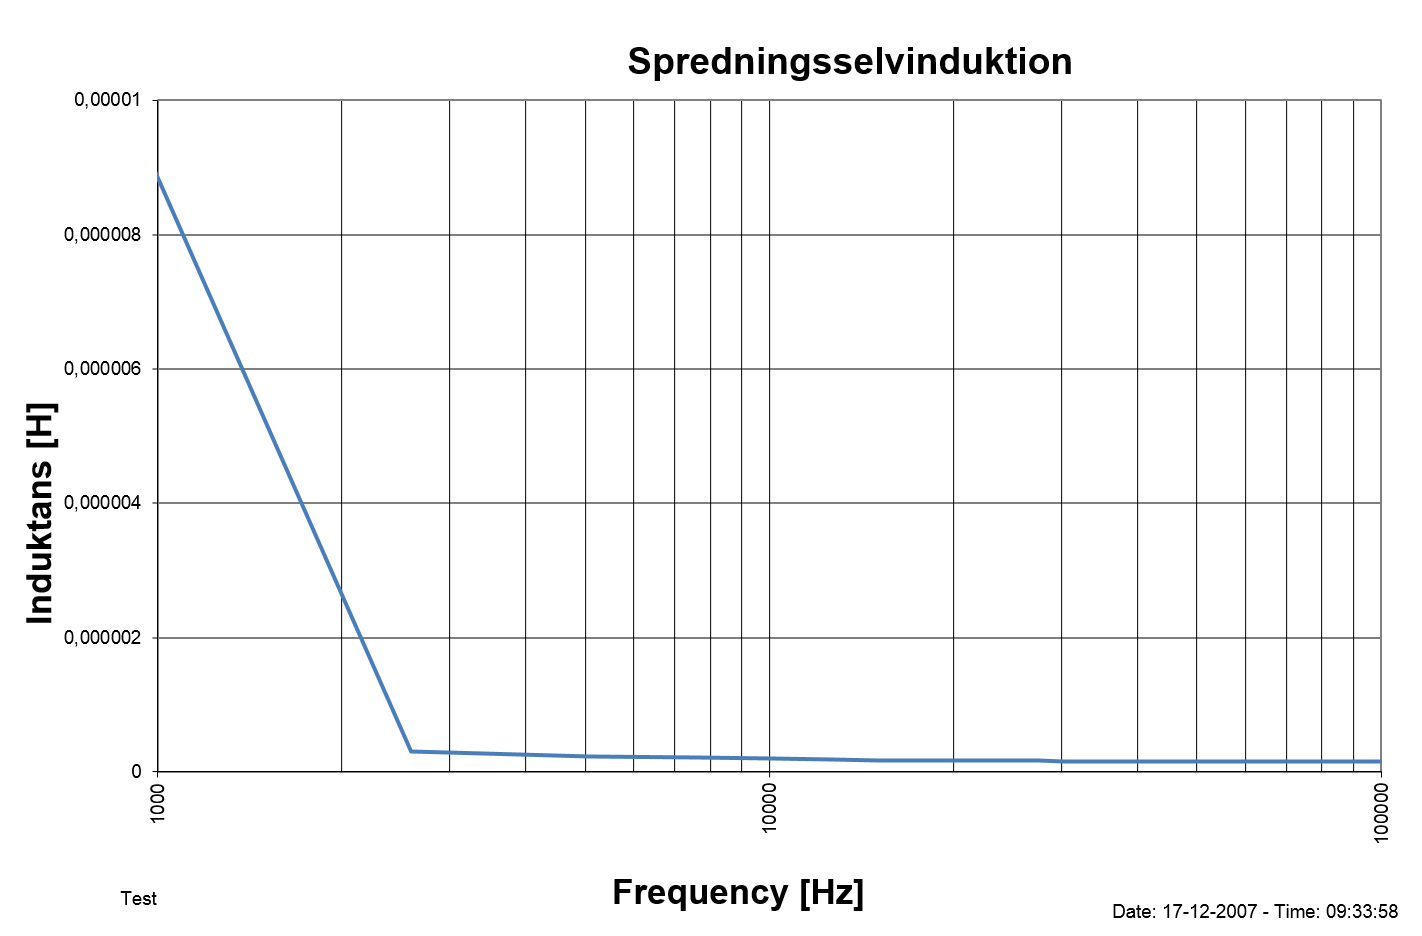
\includegraphics[max width=0.7\linewidth]{/tex/2iteration/billeder/Spredningsselvinduktion.png}
	\caption{Målt spredningsselvinduktion i transformator}
	\label{fig: leakageinductance}
\end{figure}
\noindent Denne graf er fået ud fra et frekvenssweep fra 1kHz til $100\kilo Hz$. Ved de $100\kilo Hz$ er spredningsselvinduktionen på $152\nano H$, hvilket er den værdi der bruges. 

\section{Diode}
For at mindske tabet i konverteren skal spændingsfaldet over dioden helst være så lille som muligt. Der skal dog sørges for, at dioden kan holde til den spænding, der ligger over den, når transistoren er on. Denne breakdown voltage er den maksimale indgangsspændingen plus udgangsspændingen. Faktoren på $1.3$, der ganges på, er en sikkerhedsmargin på $30\percent$:
\begin{equation} \label{Vd_break}
Vd_{break} = (V_{out}+V_{inmax}) \cdot 1.3 = 92.3V
\end{equation}
Yderligere skal dioden kunne holde til RMS strømmen på udgangen på de $3.36A$ og en peakstrøm på $5.53A$.
Schottky dioden NTSV30120CT er valgt til 2. iteration med en breakdown voltage på $120V$. Dioden kan klare en continuos strøm $5A$ og en peakstrøm på $30A$ per device. Hele devicet er med 2 dioder, og da der her kun benyttes én af dem, er det i stedet en peakstrøm på $15A$, der er maksimum. Derudover kan dens spændingsfald aflæses i databladet til ca. $0.5V$ ved $125\degreeCelsius$ og $3.36A$. 

\section{MOSFET}
MOSFET'en skal først og fremmest kunne holde til den spænding, der vil ligge over drain-source, når den er off. Ved en flyback er det den maksimale indgangsspænding plus den spænding der bliver reflekteret tilbage til primærviklingen fra sekundærviklingen. Det vil sige udgangsspændingen samt diodens spændingsfald. Derudover er der lagt en margin på $30\percent$ oveni ligesom ved dioden. Det er for at tage højde for de peakspændinger, spredningsselvinduktionen giver anledning til. Det sikrer også mod andre ringninger, der kommer af designets parasitter.  
\begin{equation} \label{Vds_break}
Vds_{break} = (V_{inmax}+(V_{out}+V_D)) \cdot 1.3 = 92.95
\end{equation}
Yderligere skal den valgte MOSFET kunne holde til RMS strømmen i primærviklingen på $3.02A$ samt peakstrømmen på $5.64A$.
Til 2. iteration er IRFB23N15 valgt.(datasheet henvisning) Den kan holde til Vds på $150V$ og en continous drain strøm på $17A$ samt en peak på $92A$, hvilket er rigeligt. Derudover en Rds(on) modstand på ca. $113\milli \ohm$ ved $50\degreeCelsius$. 

Det er en MOSFET, som vil kunne fungere i designet, men som også kan optimeres på on modstand og kapacitet på et senere tidspunkt, hvis tabet ender med at være for stort. 

\section{Udgangskondensator}
Som udgangskondensator er valget faldet på 4 parallelle kondensatorer på $56\micro F$ af typen .. Dette var den film kondensator med højest kapacitet Terma havde til rådighed. Det vigtige her, er at det er en film kondensator, da de typisk har ret præcise kapaciteter samt en lav ESR modstand. Når kondensatorer ikke længere anses som ideele, vil der i virkeligheden både være en ESL induktans og en ESR modstand. Ækvivalentdiagrammet for en kondensator vil derfor se ud som på figur~\ref{fig: con_equi} 
\begin{figure}[H]
	\center
	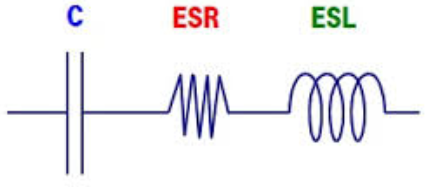
\includegraphics[max width=0.7\linewidth]{/tex/2iteration/billeder/Kondensator_equivalent.png}
	\caption{Ækvivalentdiagram for kondensatorer}
	\label{fig: con_equi}
\end{figure}
I nogle datablade kan disse parasitkomponenter slås op, det er dog ikke tilfældet for denne kondensator. Med hensyn til ESR modstanden, bliver denne af og til ikke oplyst for film kondensatorer, da den er lav ved denne type, i forhold til for eksempel en elektrolyt. 
Med hensyn til induktansen kan den estimeres ved en hovedregel, der siger, $1\nano H$ per $\milli m$. Denne kondensator har $4\centi m$ lang og induktansen estimeres dermed til $40\nano F$. Med 4 kondensatorer i parrallel giver det dermed en samlet induktans for udgangskondensatoren på:
\begin{equation} \label{ESL}
C_{ESL} = ((40\nano F)^{-1} \cdot 4)^{-1} = 10\nano F
\end{equation}

\subsection{Test af kondensator}

For at få ESR modstanden og den præcise ESL induktans, måles disse med impedansmåleren, som også blev benyttet til måling af transformatoren. Opstillingen ses på figur~\ref{fig: cap}, men er den samme som tidligere, hvor transformatoren er skiftet ud med en af kondensatorerne. 
\begin{figure}[H]
	\center
	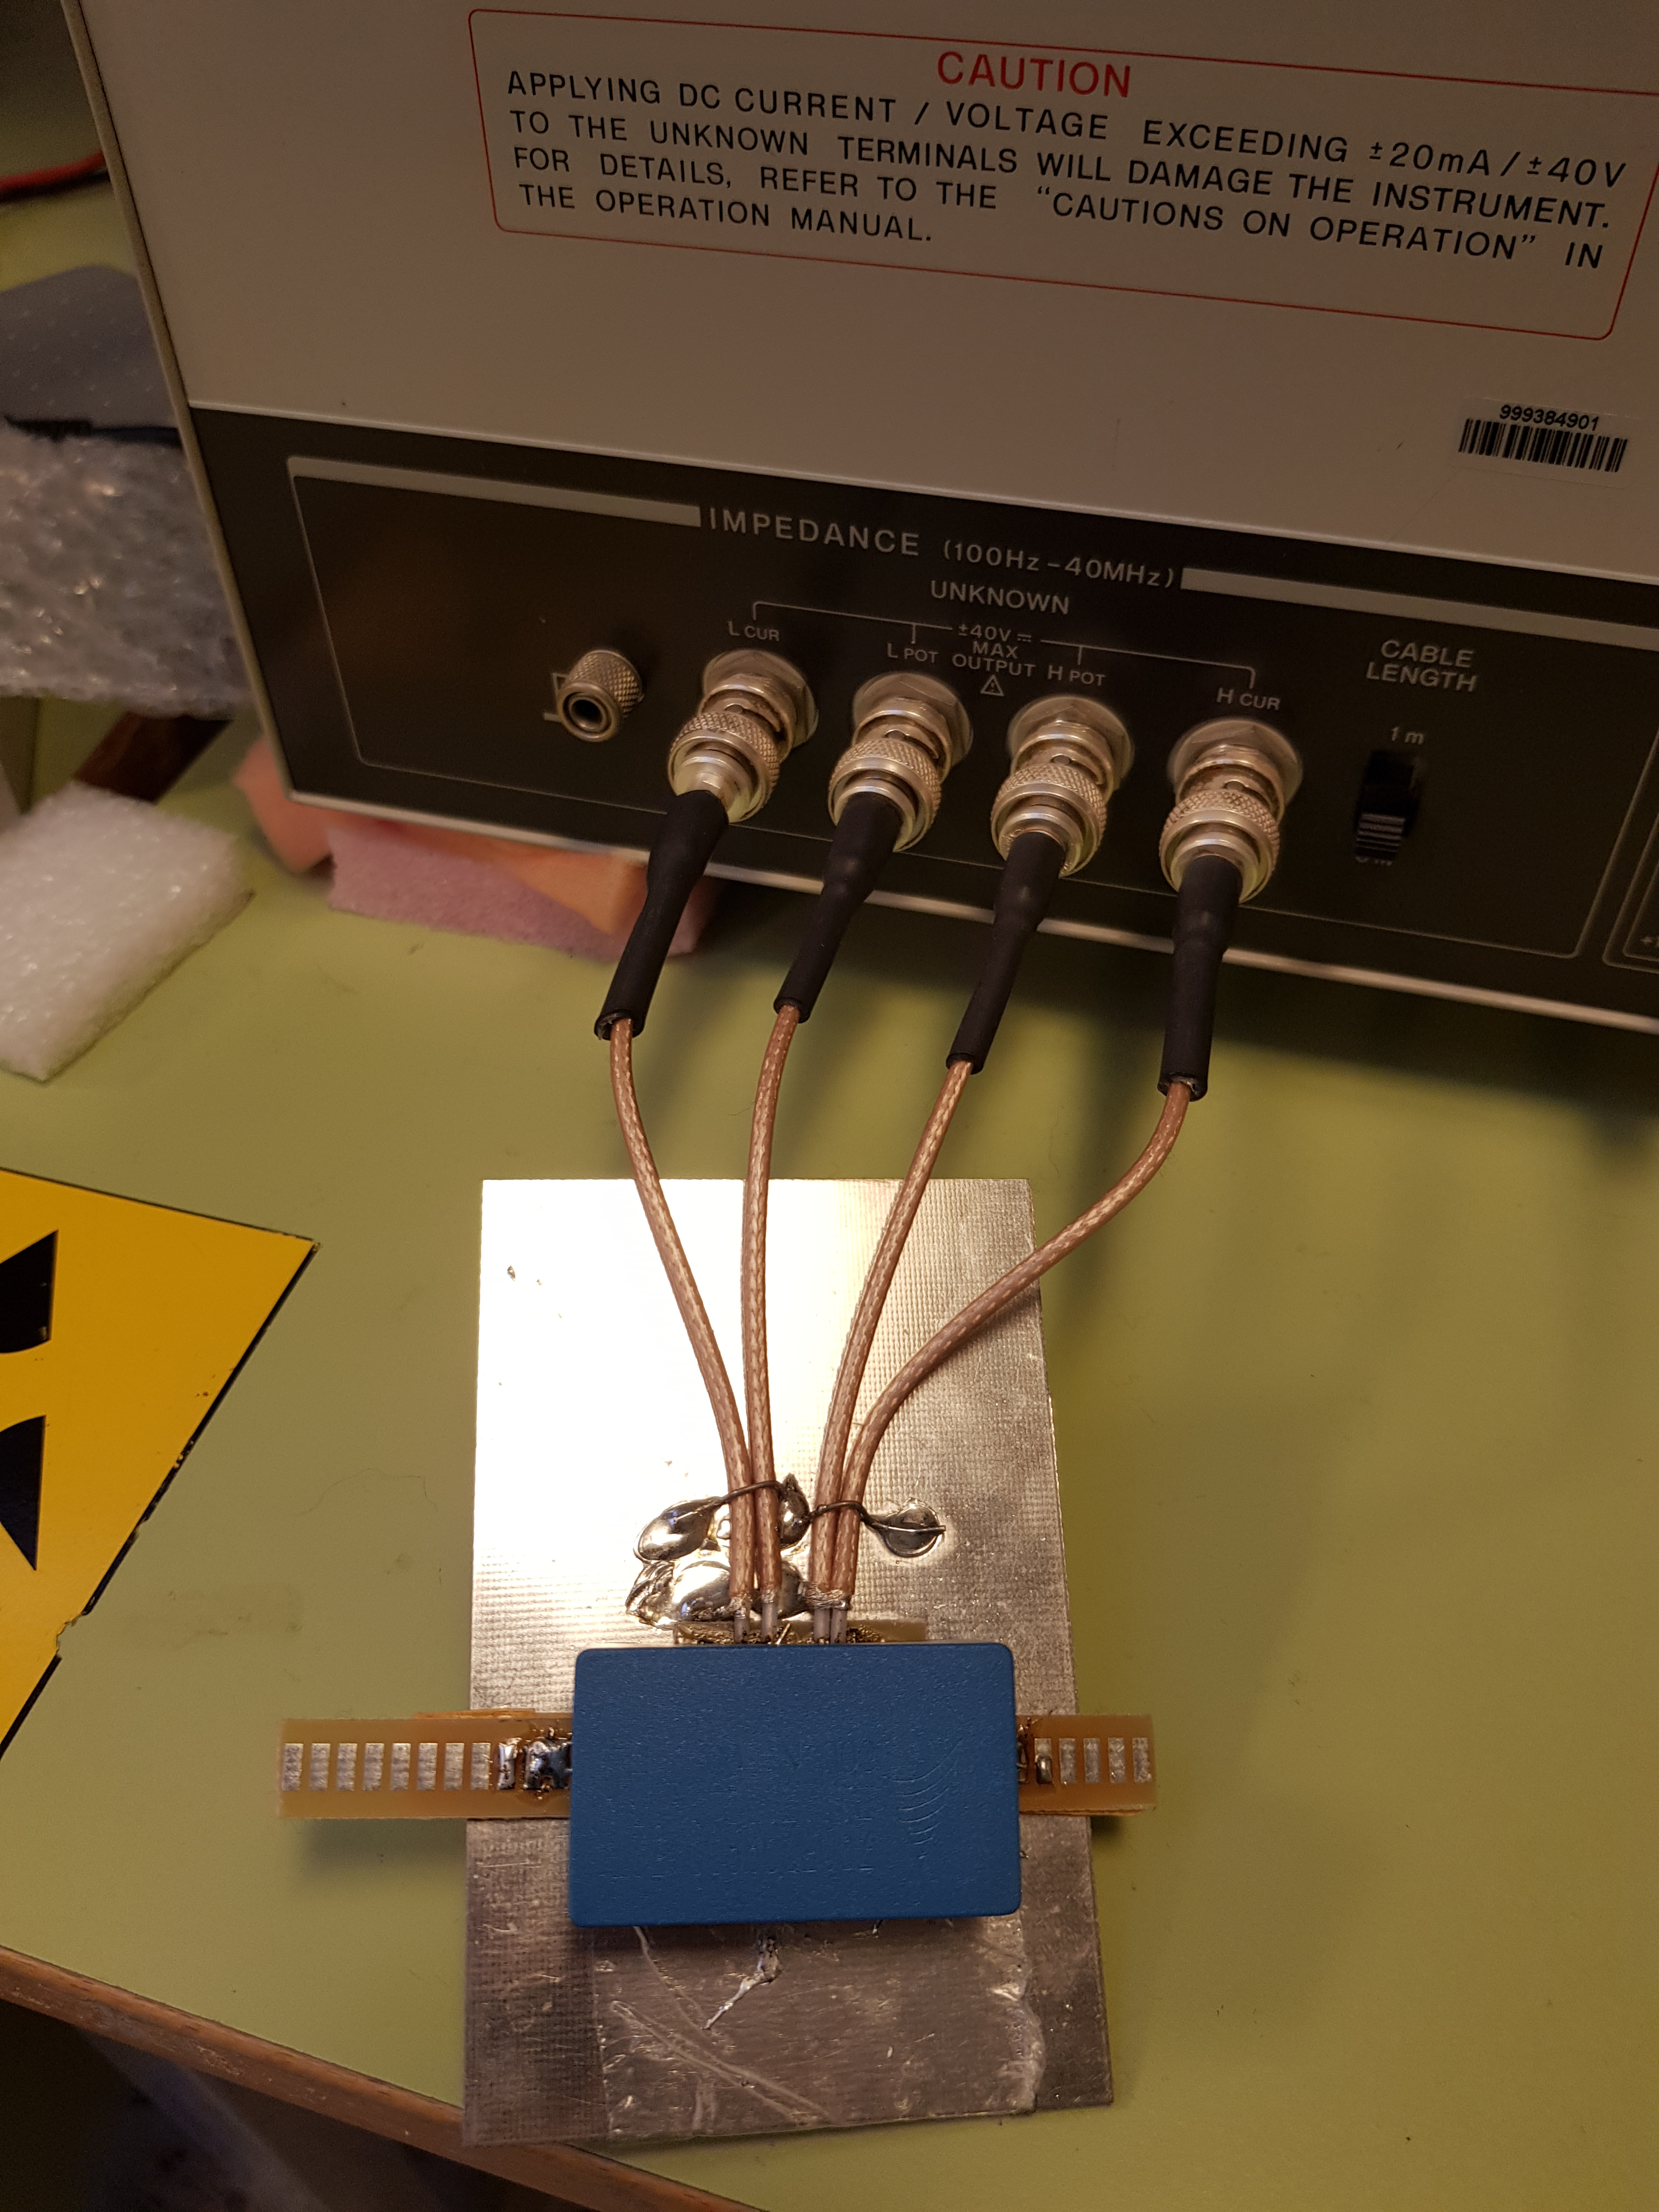
\includegraphics[max width=0.7\linewidth]{/tex/2iteration/billeder/Udgangskondensator_impedansmaling.jpg}
	\caption{Test af udgangskondensator}
	\label{fig: cap}
\end{figure}
Ligesom ved transformatoren benyttes 4-wire teknikken, for at undgå ekstra parasitter. På figur~\ref{fig: captest} ses grafen der er tegnet ud fra målingen. De enkelte målepunkter kan findes i Excel dokumentet \cite{Kondensator_impedans.xlsx}
\begin{figure}[H]
	\center
	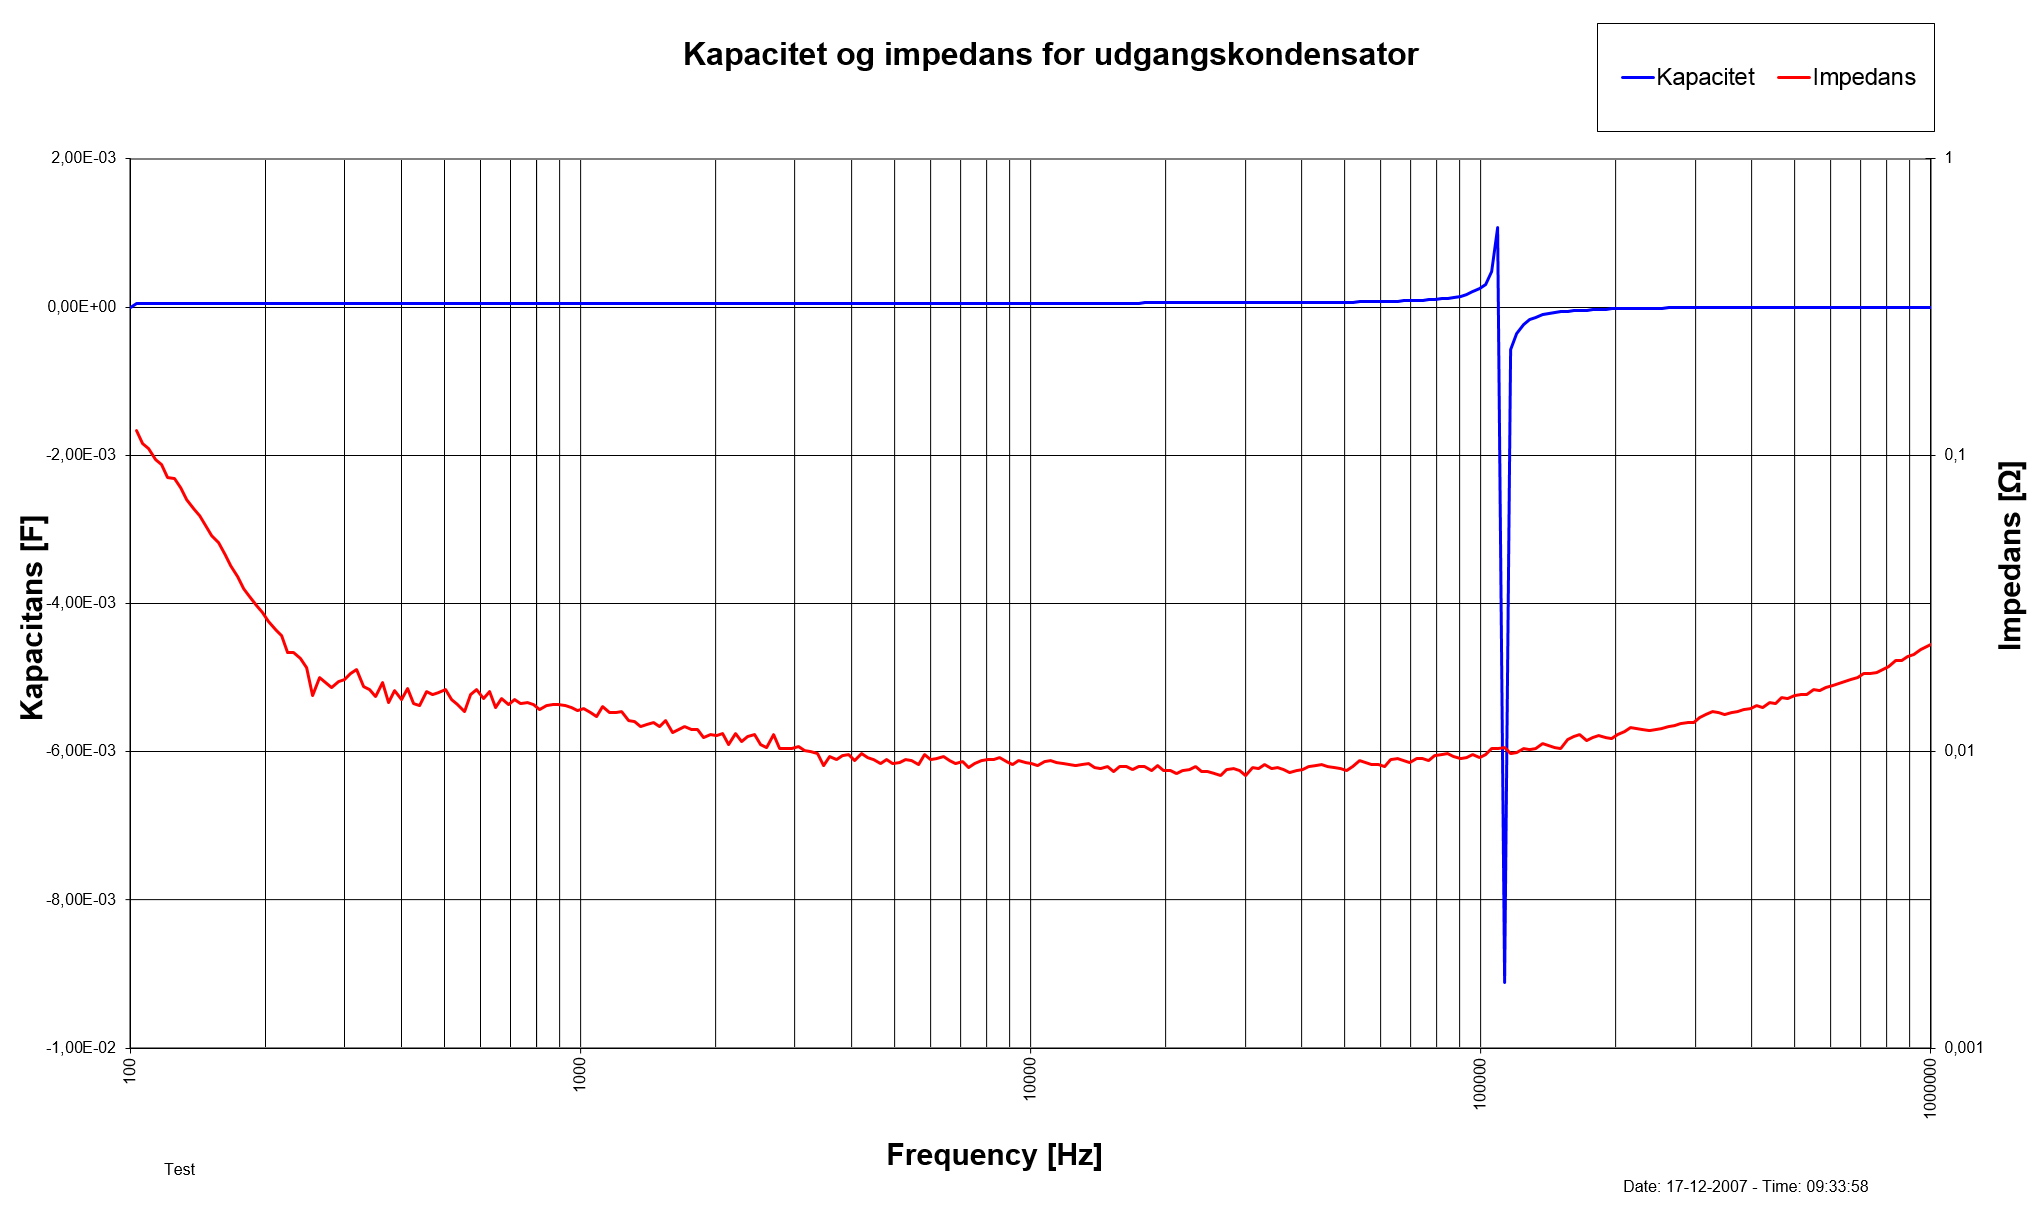
\includegraphics[max width=0.9\linewidth]{/tex/2iteration/billeder/Kondensatortest.png}
	\caption{Kapacitet og impedans for udgangskondensator}
	\label{fig: captest}
\end{figure}
Det ses tydeligt at resonantfrekvensen for det induktive og kapacitive i kondensatoren ligger lidt over de $100\kilo \hertz$, mere præcis ved $108\kilo \hertz$. 


\noindent Da der i projektet bruges en switchfrekvens på $100\kilo \hertz$, er en resonantfrekvens på $108\kilo \hertz$ ikke helt optimal. Det betyder, at der ved de $100\kilo \hertz$, formodentligt ikke vil være præcis den kapacitet der forventes. Det er dog stadig denne kondensator, der benyttes i 2. iteration. Skal der senere optimeres på dette, kan resonantfrekvensen rykkes længere op i frekvens. Det kan enten gøres ved at finde en lignende kondensator med mindre ESL induktans eller finde en kondensator med lavere kapacitet og sætte flere i parrallel end de nuværende 4.


\noindent Ved resonantfrekvensen kan ESR modstanden nogenlunde aflæses, da det kapacitive og induktive her udligner hinanden. Det vil sige, at kun ESR modstanden står tilbage, hvilket i dette tilfælde aflæses til ca. $10\milli \ohm$. 
ESL modstanden kan udregnes ud fra resonantfrekvensen og kapaciteten på de $56\micro F$:
\begin{equation} \label{CESL}
C_{ESL} = \frac{1}{4 \cdot \pi^{2} \cdot {f_{res}}^{2} \cdot C_{out}} = 38.78\nano H
\end{equation}
Hvilket stemmer meget godt overens med det estimerede på de $40\nano F$.
Det betyder, at der med de 4 kondensatorer i parallel vil være en samlet ESL induktans på: 
\begin{equation} \label{CESLtot}
C_{ESLtot} = ((38.78\nano F)^{-1} \cdot 4)^{-1} = 9.70\nano F
\end{equation}
Samt en samlet ESR modstand på:
\begin{equation} \label{CSRtot}
C_{ESRtot} = ((10\milli \ohm)^{-1} \cdot 4)^{-1} = 2.5\milli \ohm
\end{equation}

\section{Input filter}
Input filtreret har som sådan ikke været en del af projektet, da det er blevet givet af Terma. Dette blev gjort, så der kunne fokuseres andetsteds. 

\noindent Herunder beskrives filtret dog stadig, så der gives forståelse for, hvordan det er designet og hvad det bruges til.

\noindent \cite{Inputfilter} Et input filter er nødvendigt i switch mode power supplies. For det første skal det sikre imod den elektromagnetiske interferens, der bliver genereret fra switching. Hvis denne interferens får lov at komme ud på forsyningsnetværket, vil det påvirke andet udstyr, hvilket selvfølgelig ikke er hensigtsmæssigt. Mængden af  tilladeligt EMI (elektromagnetisk interferens) er fastlagt af standarder verden over, så hvis ikke produktet overholder dette, kommer det aldrig på markedet.

\noindent Udover EMI skal filtret også sikre, at højfrekvent spænding fra forsyningsnettet, ikke når outputtet for power supplien.\fxnote{Converteren?} 

Det er i dette projekt gjort med et parallel dæmpet filter. Det består af et LC led, der giver en overordnet resonant frekvens. I sig selv, bør det kunne sikre sig imod de 2 punkter beskrevet ovenfor. Problemet i kun at bruge denne del, ligger ved knækfrekvensen\fxnote{Find en graf for et anden ordensfilter}. Når filtret er udæmpet, som det er ved et LC, kan der komme stor forstærkning ved cut off frekvensen, og derfor forstærke støjen ved den frekvens istedet. Det betyder at der gerne skal ligge en stor dæmpning ved frekvensen. Med en lille dæmpningsfaktor fås et stort gain ved cut off frekvensen og omvendt. En dårlig dæmpningsfaktor kan give resten af systemet en dårligere performance. Det kan gå ind og påvirke overføringsfunktionen til reguleringsloopet og på den måde få systemet til at oscillere. Hvis der sørges for, at udgangsimpedans kurven for input filtret ligger meget under impedanskurven for konverteren, vil konverterens loop gain ikke blive ændret det store. Det vil sige, at det er vigtigt at holde peak impedansen nede for filtret, for at undgå oscillerings problemer forårsaget af inputfiltret.     

Det er her, det parallelle led kommer ind i billedet. Det består af en modstand i serie med en kondensator. Meningen med modstanden er, at reducere udgangs peak impedancen af filtrets cutoff frekvens. Samtidig vil kondensatoren i serie med modstanden sørge for, at blokere DC delen af inputspændingen og derfor mindske effekttabet i modstanden. Denne kondensator skal have en mindre impedans end modstanden ved resonantfrekvensen og en større kapacitans end filter kapaciteten. Dette vil gøre, at cutoff frekvensen af R-L filtret ikke påvirkes af kondensatoren. På figur~\ref{fig: Inputfilter} ses hele filtret givet af Terma.    
\begin{figure}[H]
	\center
	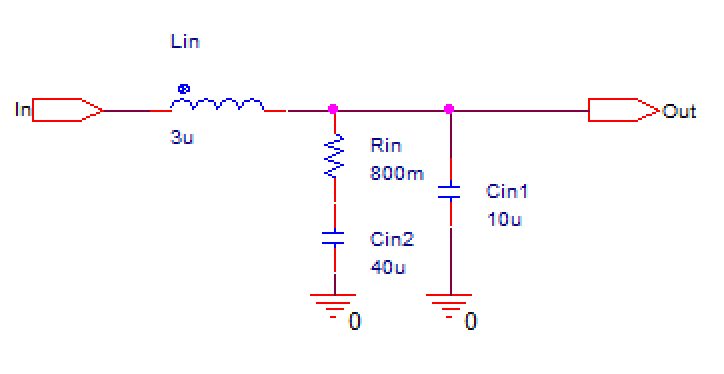
\includegraphics[max width=0.7\linewidth]{/tex/2iteration/billeder/Inputfilter.png}
	\caption{Inputfilter}
	\label{fig: Inputfilter}
\end{figure}
Det ses, at filtret har en overordnet knækfrekvens på:
\begin{equation} \label{fc}
f_c = \frac{1}{2 \cdot \pi \cdot \sqrt{3\micro H \cdot 10\micro F}} = 29.06kHz
\end{equation}
Samtidig kan det konkluderes, at selve kapaciteten på $C_{in2}$ er 4 gange større end $C_{in}$ samt impedansen bliver:
\begin{equation} \label{XC2}
X_{Cin2} = \frac{1}{2 \cdot \pi \cdot 40\micro F \cdot 29.06kHz} = 0.137\ohm
\end{equation}
Hvilket er mindre end modstanden på $0.8\ohm$. Det vil sige, at filtret opfylder kriterier opstillet ovenfor.

\section{Tab}
Her vil tabene for komponenterne i 2. iteration blive udregnet

\subsection{Transformatortab}
Transformatortabet kan deles op i 2 dele. Et kernetab og et kobbertab. Det beregnes herunder

\subsubsection{Kernetab}
Selve kernetabet afhænger af kernematerialet, induktans og strømmen der løber i viklingerne. Først udregnes delta B.
\begin{equation} \label{DeltaB}
\Delta B = \frac{L \cdot I_{pk21}}{N \cdot A_0} = 263.59\milli T
\end{equation}
For at få peak fluxen divideres med 2. Med den kan tabet i kernen per $\frac{\kilo W}{m^3}$
\begin{equation} \label{B}
B = \frac{\Delta B}{2} = 131.79\milli T
\end{equation}
Med den information kigges i databladet under kurven for power loss som funktion af peak flux density.
\begin{figure}[H]
	\center
	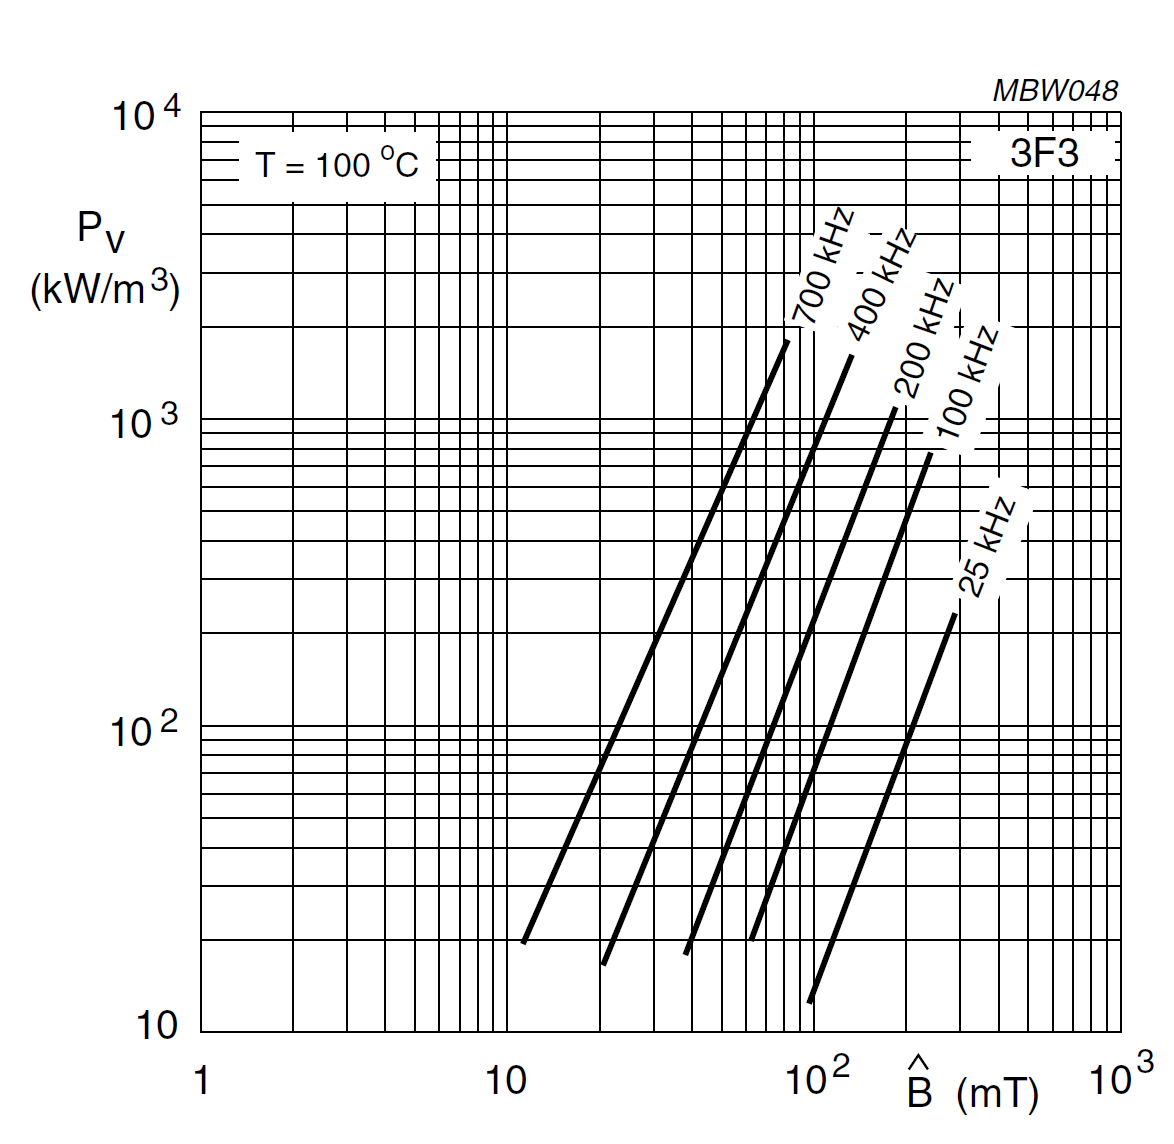
\includegraphics[max width=0.7\linewidth]{/tex/2iteration/billeder/Powerloss.png}
	\caption{Power loss som funktion af peak flux density}
	\label{fig: Powerloss}
\end{figure}
Her ses på de $100\kilo Hz$ ved de ca. $132\milli T$. Det aflæses til et power loss på ca. $150\frac{\kilo W}{m^3}$.
Det samlede kernetab fås med denne værdi ganget med den effektive volumen for RM8 kernen.
\begin{equation} \label{DeltaB}
P = P_V \cdot V_e = 366\milli W
\end{equation}
Dette passer forholdsvis pænt med det simulerede tab i kernen på $310\milli W$.

\subsubsection{Kobbertab}
Kobbertabet i transformatoren opstår på grund af modstanden i de kobbertråde den er viklet med. Den modstand deles op i to bidrag - en DC-modstand og en AC-modstand. DC-modstanden bestemmes ud fra længden og tykkelsen af tråden, mens AC-modstanden afhænger af indtrængningsdybden og trådens diameter. 

\paragraph{AC-modstand}
AC-modstanden i viklingerne opstår på grund af, det magnetfelt kobbertrådene ligger i. Magnetfeltet skaber en hvirvelstrøm der løber i trådene. Hvirvelstrømmen vil derfor være et ekstra bidrag, til den driftsstrøm der bliver sendt ind i transformatoren. Dette vil komme til udtryk, som et ekstra bidrag til den samlede modstand i viklingerne. 

AC-modstanden afhænger af indtrængningsdybden og trådens diameter. Hvis diameteren er tilpas lille i forhold til indtrængningsdybden, vil  hvirvelstrømmene i tråden udligne sig selv, og derved ikke bidrage til tabet. Er tråden til gengæld for tyk i forhold til indtrængningsdybden, vil det resultere i en hvirvelstrøm, der løber i hele trådens længde. 

Måden man bestemmer AC-modstanden, er ud fra princippet \textit{Eddy Current Losses}. Det siger at forholdet mellem AC- og DC-modstanden, kan bestemmes ud fra forholdet mellem trådens diameter og indtrængningsdybden. Disse forhold er skitseret på figur~\ref{fig:Eddy_current_losses}\cite{eddy_current_losses}. Her ses det også, at AC-modstanden afhænger af hvor mange lag man vikler på transformatoren. 

\begin{figure}[H]
	\center
	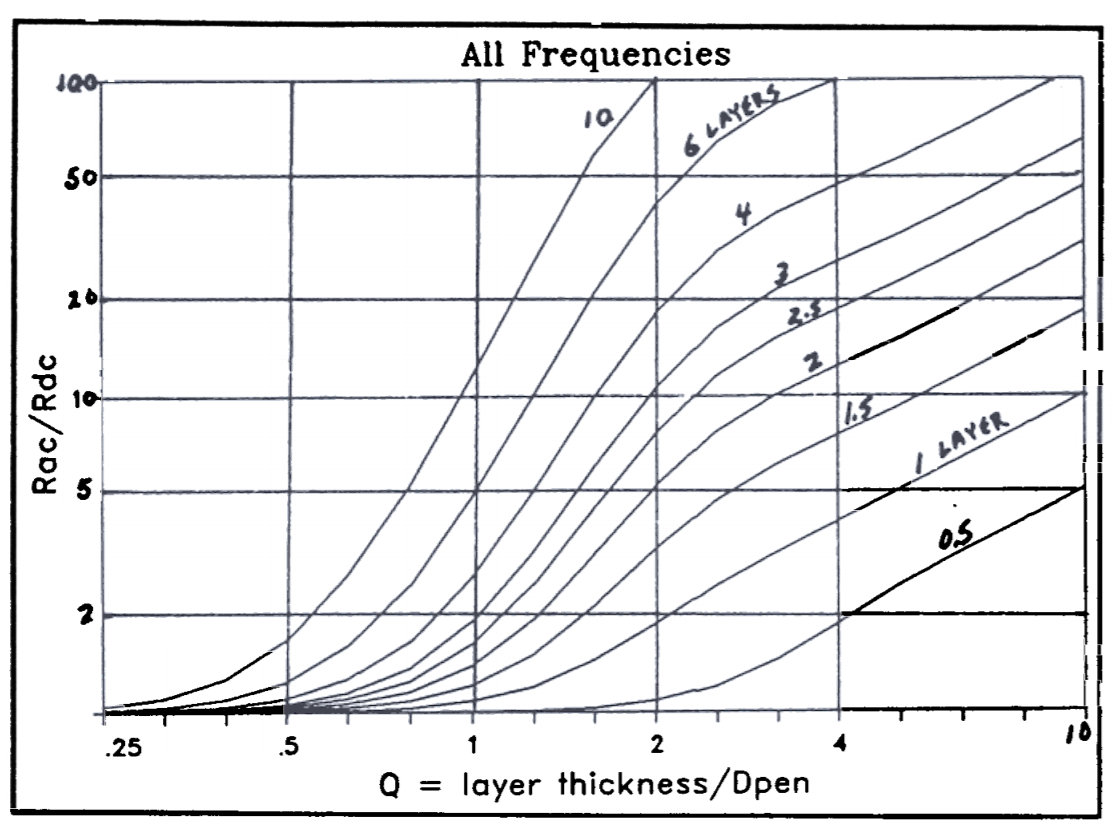
\includegraphics[max width=0.7\linewidth]{/tex/2iteration/billeder/Eddy_current_losses.PNG}
	\caption{Eddy Current Losses}
	\label{fig:Eddy_current_losses}
\end{figure}

Dette er kompliceret at regne for en flyback transformator, og vil derfor ikke blive gjort i dette projekt. Derfor vil kobbertabet i transformatoren, kun være en estimering af det samlede kobbertab.

\paragraph{DC-modstand}
For at beregne DC-modstanden, udregnes først omkredsen af kerneformen. Transformatoren er viklet på en RM8. Denne form har i følge databladet en indre diameter på $9.95mm$ og en ydre diameter på $16.9mm$. For at finde en gennemsnitslængde på tråden, beregnes et gennemsnit af formens diameter, for derefter at beregne omkredsen af formen.
\begin{equation} \label{Diameter}
D = \frac{9.95mm \cdot 16.9mm}{2} = 13.43mm
\end{equation}
\begin{equation} \label{Omkreds}
O = D \cdot \pi = 4.23cm
\end{equation}

Ud fra omkredsen på kerneformen, kan længden af hver kobbertråd beregnes, ved at gange med antallet af vindinger for en vikling. For den viklede transformator er $N=19$.
\begin{equation} \label{Lengde}
l = O \cdot N = 80.13mm
\end{equation}

Diameteren på kobbertråden er valgt til $0.425mm$. Denne diameter er inkl. lakering. Ud fra et tabelopslag ved Grade 2\cite{wire-diameter}, aflæses den nominelle kobberdiameter af denne tråd $0.375mm$.
Ud fra denne diameter beregnes trådens tværsnitsareal.
\begin{equation} \label{kobber-areal}
A_{cu} = \frac{0.375mm}{2}^2 \cdot \pi = 0.11mm^2
\end{equation}

For at beregne DC-modstanden bruges kobbers resistivitet ved $100\degreeCelsius$, for at regne worst case. Denne opslås til $\rho=2.204\cdot 10^{-8}\ohm \cdot m$. Nu kan hver enkelt tråds DC-modstand bregnes ud fra trådens længde, samt tværsnitsareal.
\begin{equation} \label{dc1-modstand}
R_{DC1} = \frac{l \cdot \rho}{A_{cu}} = 159.91\milli\ohm
\end{equation}

Transformatoren er viklet med tre tråde i parallel ved både primær- og sekundærviklingen. Derfor beregnes den samlede modstand, ved at regne parallelmodstanden:
\begin{equation} \label{dc-modstand}
R_{DC} = ((R_{DC1})^{-1} \cdot 3)^{-1} = 53.3\milli\ohm
\end{equation}

Kobbertabet i transformatoren, kan nu beregnes ved RMS-strømmene i primær- og sekundærviklingerne. Hvor $I_{RMSp} = 3.02A$ og $I_{RMSs} = 3.36A$.
\begin{equation} \label{dc-tab-pri}
P_{cuP} = (I_{RMSp})^2 \cdot R_{DC} = 0.486\milli\watt
\end{equation}

\begin{equation} \label{dc-tab-sek}
P_{cuS} = (I_{RMSs})^2 \cdot R_{DC} = 0.602\milli\watt
\end{equation}

\section{Simulering}

I dette afsnit laves simuleringen for det samlede kredsløb i 2. iteration. 
Selve simuleringsdokumentet er delt op i blokke for at gøre det mere overskueligt. 


\noindent Kigges der på det yderste trin på figur~\ref{fig: simtop}, ses blot indgangsspændingen på 26V og udgangsloaden, der er sat op til $8.4\ohm$.
\begin{figure}[H]
	\center
	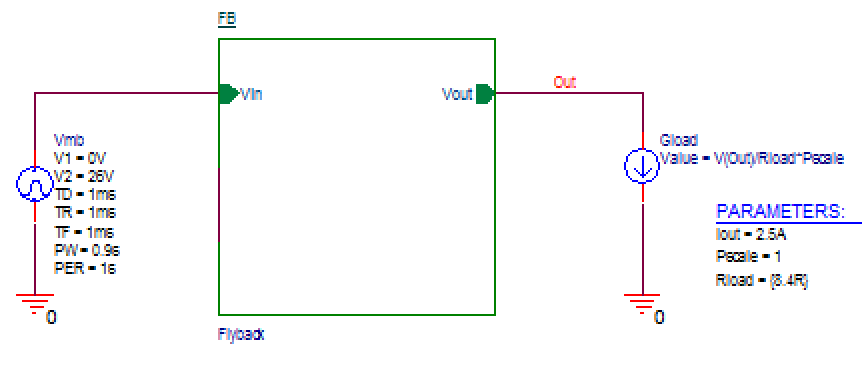
\includegraphics[max width=0.7\linewidth]{/tex/2iteration/billeder/Simulering_2iteration_top.png}
	\caption{Yderste blok af simulering}
	\label{fig: simtop}
\end{figure}
Imellem er blokken "Flyback". Heri er selve kredsløbet. Dykkes der ind i denne blok fås det der ses på figur~\ref{fig: simfly} 
\begin{figure}[H]
	\center
	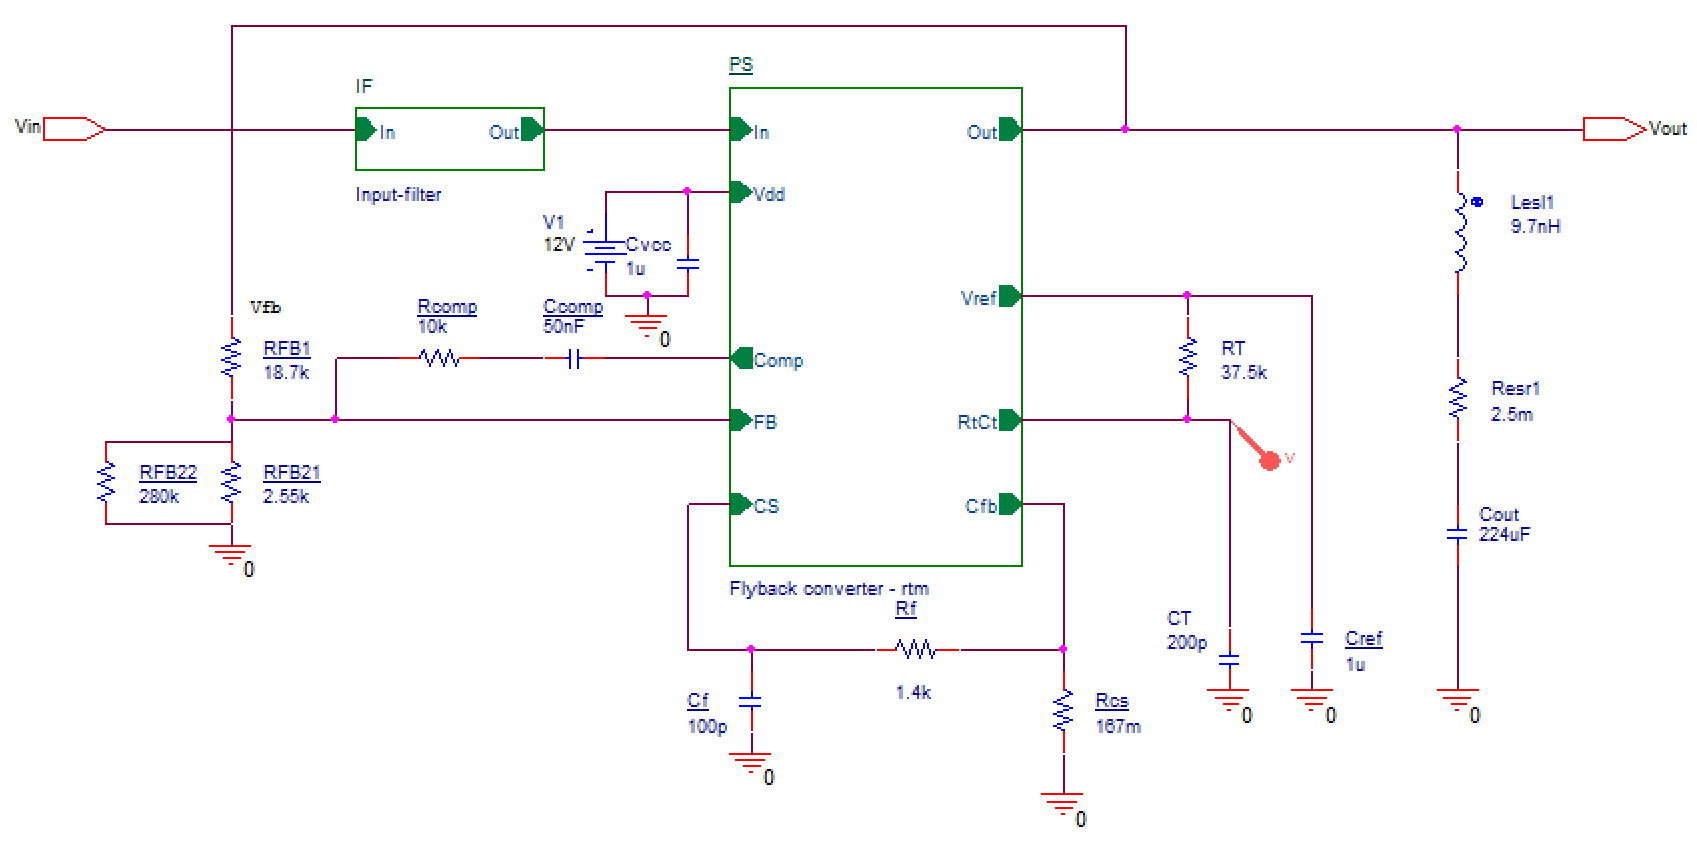
\includegraphics[max width=0.7\linewidth]{/tex/2iteration/billeder/Simulering_2iteration_flyback.png}
	\caption{Flyback blok}
	\label{fig: simfly}
\end{figure}
Her ses yderligere 2 blokke hhv. Inputfilter og flyback converter. Ud over disse blokke ses de komponenter, der er brugt til at få PWM controlleren til at køre efter hensigten. Selve controlleren ligger inde i flyback converter blokken. Værdierne og forklaringen af komponenterne blev gennemgået i analyse afsnittet om PWM controlleren??
Desuden ses output kondensatoren med de udregnede parasitter også.


\noindent Blokken for inputfiltret er allerede vist tidligere under forklaringen af denne, så den vises ikke igen. Til gengæld ses indholdet af Flyback converter blokken på figur~\ref{fig: simflycon}. 
\begin{figure}[H]
	\center
	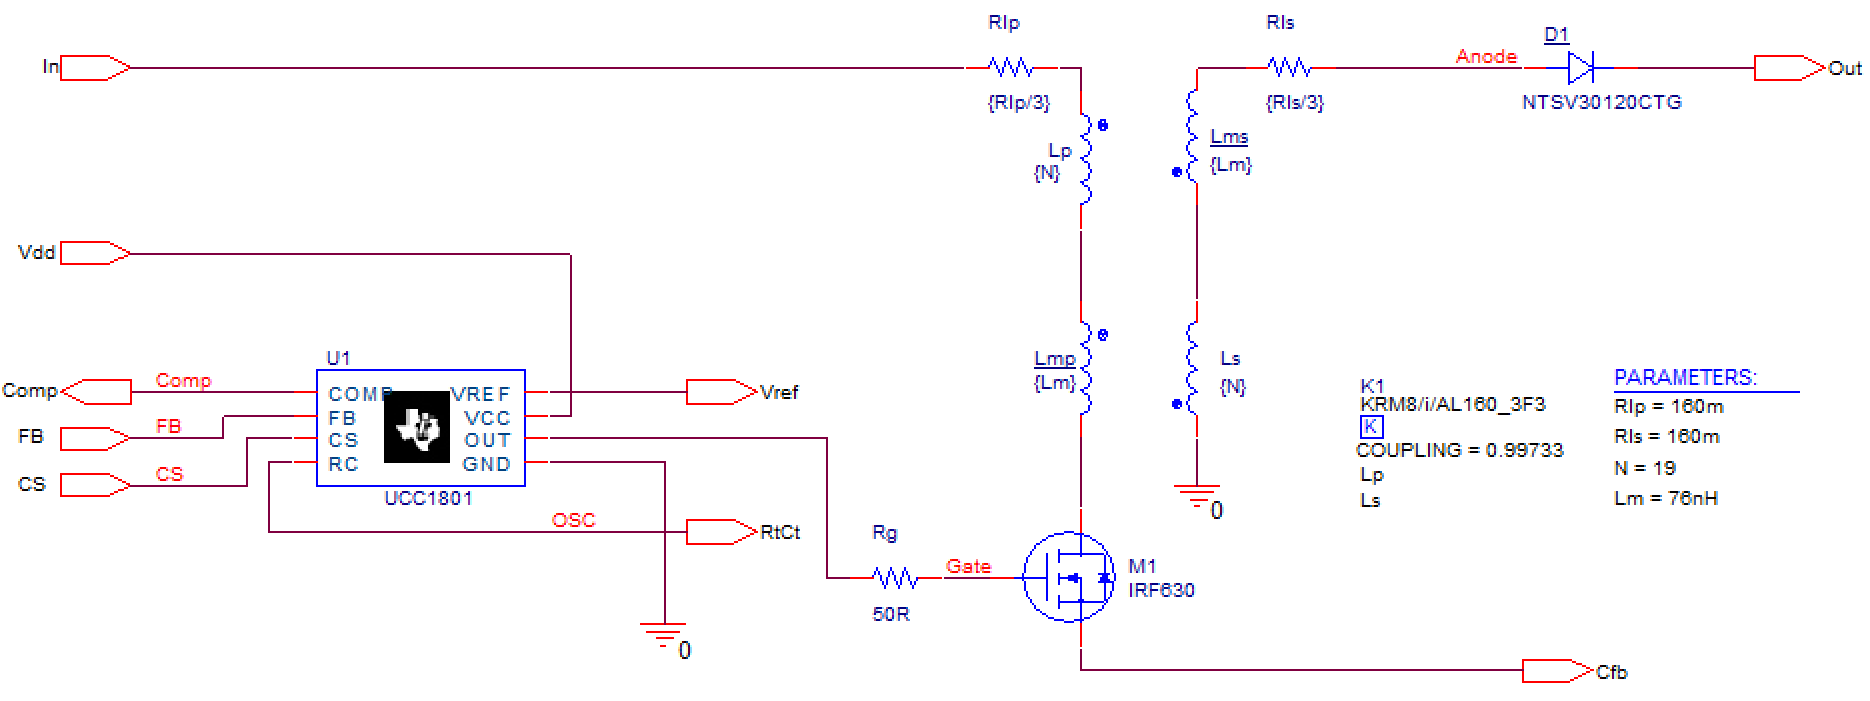
\includegraphics[max width=0.7\linewidth]{/tex/2iteration/billeder/Simulering_2iteration_flycon.png}
	\caption{Flyback converter blok}
	\label{fig: simflycon}
\end{figure}
Heri ses selve PWM controlleren UCC1801, som der er trukket en model ind for. \cite{??}. Også MOSFET'en og Dioden er der trukket modeller ind for. Ved MOSFET'en har det ikke været muligt at finde den præcise model. Derfor er IRF630 modellen istedet brugt, da det er vurderet, at den minder en del om den. \cite{IRF630MOSFET} 
Yderligere ses transformatoren, hvor både spredningsselvinduktion og kobbermodstanden i ledningerne er tegnet med samt kernemodellen for 3F3 er trukket ind.

\subsection{Constant load}
Ved constant load simuleringen simuleres ved en load på $8.4\ohm$, efter $20ms$ så det sikres, at der ses på den stationære udgang. Indgangsspændingen er sat til 26V.
Første plot af denne simulering ses på figur~\ref{fig: simflycon}. Her ses både strøm og spænding på udgangen.
\begin{figure}[H]
	\center
	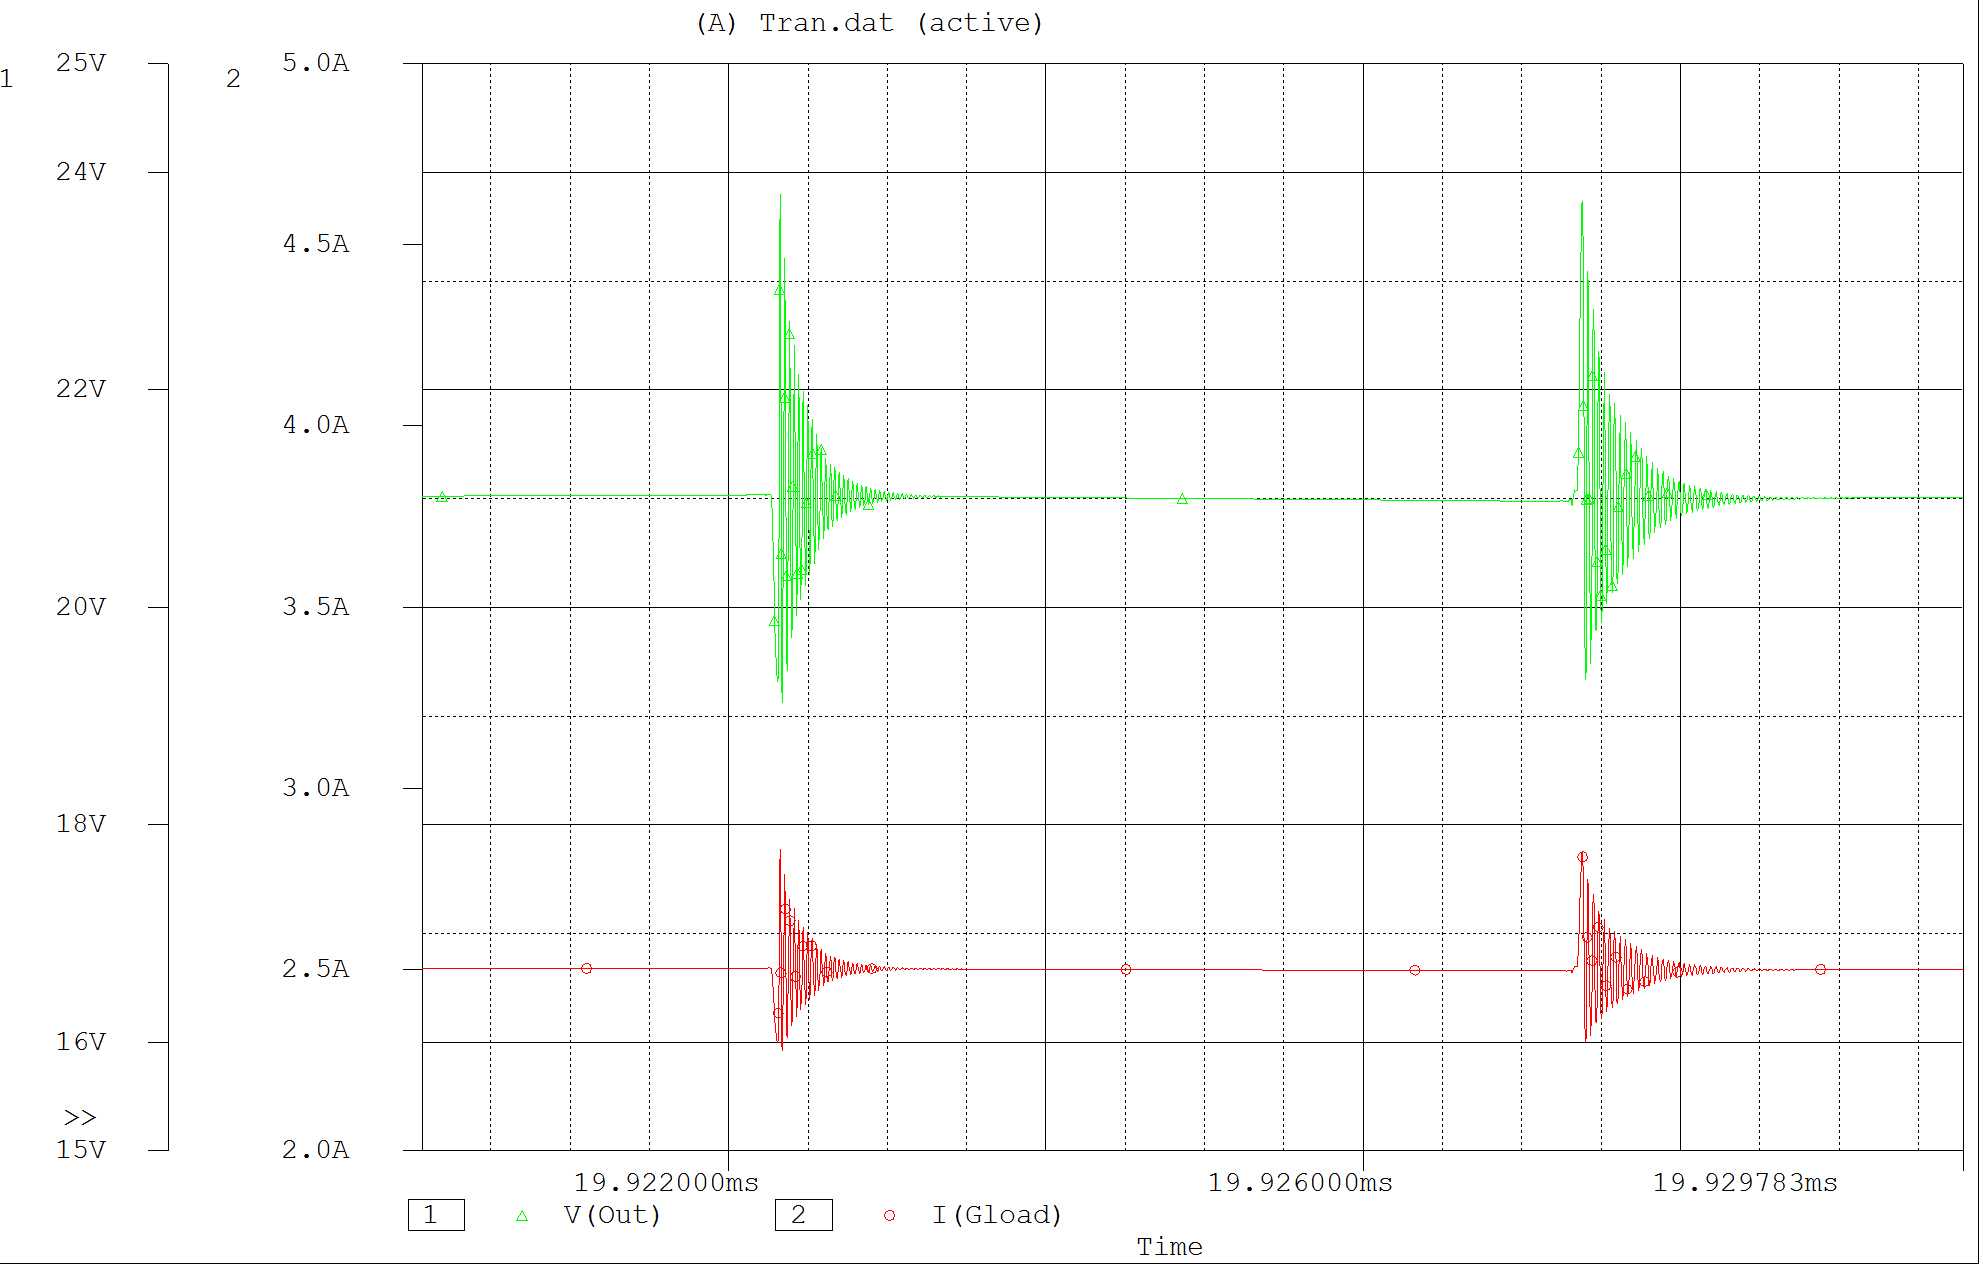
\includegraphics[max width=0.7\linewidth]{/tex/2iteration/billeder/Simudgang.png}
	\caption{Simulering af udgang}
	\label{fig: simudgang}
\end{figure}
Her ses det at spændingen V(out) ligger på 21V, dog med svingninger hver gang der switches. Det ser altså ud til at switching transienter fra MOSFET og diode kommer til syne på udgangen. Det er samme billede for strømmen I(Gload), der ellers ligger på de forventede 2.5A.

På figur~\ref{fig: simMOSdio} ses en spændingsperiode for drain benet på MOSFET'en samt dioden. 
\begin{figure}[H]
	\center
	\includegraphics[max width=0.7\linewidth]{/tex/2iteration/billeder/SIMMOSFETdiode.png}
	\caption{Simulering af spænding over diode og drain ben på MOSFET}
	\label{fig: simMOSdio}
\end{figure}
Det ses, at når transistoren (rød kurve) går off så kommer den tidligere omtalte peakspænding samt den svinger, inden den går til en stationær værdi på ca. 48V, inden MOSFET'en switches on igen. Dette stemmer fint overens med analysen hvor den stationær værdi bør ligge på 21V+26V=47V.
Peak'en er ca. 93V.
Det samme ses for dioden (grøn kurve) at når transistoren er on, vil dioden ikke være i lederetningen, og skal derfor kunne holde til den peak på ca. 80V der ses på grafen. Derudover lægger den sig på en stationær værdi på ca. 46V, hvilket igen stemmer pænt overens med de 47V.
